%!TEX root = ../thesis.tex
\chapter{Results}
\label{chap:Results}
In this Chapter, I characterise the methodology detailed in Chapter  \ref{chap:BHM} and then I applied it to the \gls{rdr2} data set (Sect. \ref{sect:DR2}). To characterise the methodology as a classifier, I measure its precision and accuracy when applied on synthetic data where the true members of the cluster are known. With this characterisation, I am able to obtain an optimal probability threshold, but only for classification purposes. Afterwards, I apply the methodology to the \gls{rdr2} and I find the candidate members of the cluster using the optimal probability threshold. Then, I compare these candidate members with those found by previous studies.

Later, I analyse the main results of this work, those that fulfil the objective: the statistical distributions that characterise of the cluster population. Then, I give the details of the spatial, velocity, luminosity and mass distributions. Finally, I end this Chapter describing the physical scenario of the evolution of the mass distribution of the Pleiades by comparing it with other mass distribution of younger and older clusters.

\section{Performance of the classifier}
\label{sect:classifier}
As mentioned earlier, the main objective of the methodology of the \gls{bhm} is the statistical characterisation of the \gls{nyc} populations. However, as a by product, it also obtains the individual membership probability distributions of the objects comprising the data set. These membership probability distributions, together with a probability threshold, allow a direct classification of the objects into cluster and field members.  The classification resulting from this procedure, as any other measured property, has an uncertainty. By evaluating this uncertainty under the results of synthetic data (in which the true members are known) we are able to measure the accuracy and precision of the classification process as a function of the probability threshold used. This section explains how an objective probability threshold can be found by maximising the accuracy of the classifier. 

To measure the accuracy of our classifier, I test it over synthetic data sets that resemble the real \gls{rdr2} data set (Section \ref{sect:RDR2}). An ideal test to our classifier will be to apply it over well known dataset in which tags of cluster and field members were already present. However, if we may have access to these tags, a classifier may not be needed. The Pleiades cluster being one of the most studied cluster in history, it is the \gls{nyc} with most of these tags (see Section \ref{sect:memberscomparison}). This is also one of the reasons for which we decided to benchmark our methodology on it. In spite of the large number of candidate members for the Pleiades clusters, the synthetic data and its true tags are still needed. The reasons are the following. First, the list of candidate members provided by the literature is not infallible. We can never be sure that this list is complete and unpolluted. Here it is important to note that the astrophysical domain of the phenomenon marks a very important distinction with common supervised classification methods. A perfect and real training set is not available. It must be created from simulations. Second, even if the most probable candidate members from the literature were used as a training set \cite[as done for example by][]{Sarro2014} the very faint end of the magnitude distribution (represented by brown-dwarfs) is still a \emph{terra incognita} where candidate members are scarce or not even exist. 

Thus, to overcome the problem of the true tags, we decided to create synthetic data sets. These synthetic true tags, and therefore the results obtained from them, rely on the assumption that our cluster and field models resemble the real data. I am aware that these models are far from perfect, but so far this assumption provides the best option. Although this assumption enable us to quantify the internal consistence (precision and accuracy) of our classifier, it does not give any indication about possible biases in the model. To explore this possibility, in the next Section, I compare our real data classification results with those of the literature.

The random nature of the synthetic data sets demands the repetition of the data sets and results. This repetitions avoid any bias caused by excursions of the random number generator (bad luck), and more importantly, they allow us to compute the uncertainty in the accuracy and precision of the classifier. As explained before, the methodology presented in this work is computing demanding. Thus, to be able to repeat at least five times the results of the synthetic data sets, we further reduce the data set size. The inference process in a data set of $10^4$ objects demands almost week of computing time. Thus, we decided that such data set provided a good compromise between computing time and number of objects. Furthermore, to provide a better estimate of the contamination rate on the results over the real \gls{rdr2} data set (the one with the $10^5$ objects) we choose to work with the $10^4$ objects with high membership probability according to \citet{Bouy2015}. Since this sample is relatively more entangled with the cluster than that of the \gls{rdr2}, we assume that the contamination rate we measure on this sample will be comparable or even higher than that hypothetically obtained over the $10^5$ \gls{rdr2}. 

Briefly, to create the synthetic data set, the procedure is the following. First, using the methodology of the previous Chapter, I obtain a sample of the posterior distribution of the parameters in the model given the $10^4$ real data set. Then, I choose the particle with highest posterior probability as the \gls{map} estimate of the posterior distribution. Using this particle positions in the parametric space, I generate five synthetic data sets of $10^4$ objects each. Then, I tag these objects according to their parent population: cluster or field. Afterwards, using the vector of synthetic values of each object, I assign their uncertainties and missing value entries (more details  below).

Finally, I run the methodology over the five synthetic data sets, and obtain a sample of the individual membership probability distributions of each synthetic object. Then, I compare the true tags with the measured ones as function of the probability threshold. 

To further test the performance of the classifier, I apply it on a synthetic data set in two different cases. In the first case the data set is one of the five synthetic ones. Thus it contains objects with missing value entries in their vector of observables.  In the second case the data set is the same as in the previous case, but this time all the objects have fully observed vectors (i.e. do not have missing value entries). The comparison of the results rendered by these two cases allows us to quantify the impact of missing values. 

Objects in the \gls{rdr2}  have full observed proper motions vectors. Since missing values appear only in the photometric entries, I only mask as missing the photometric entries of the synthetic data sets. The procedure to mask entries as missing is the following.

For each synthetic datum, I use the mask of missing entries of one of its closer neighbours in the real data set. Here, distance is measured in the euclidean sense. If I were to use the missing value mask of the nearest neighbour in the real data set, then I will obtain a biased sample in which objects with fully observed vectors will be underestimated. This is the inevitable consequence of  euclidean distances being measured in subspaces resulting from removing the dimensions of the missing entries. Since these distances are the smaller, or at most equal, to those measured in the complete space, the fully observed objects will be under represented.

The mask of missing entries is chosen from amongst the missing values of the closer neighbours in the available \glspl{cmd}: $\{K_s,J-K_s\},\{J,J-H\},\{K_s,H-K_s\},\{J,Y-J\},\{K_s,i-K_s\}$. These \glspl{cmd} comprise, in decreasing order, the bands and colours of the magnitudes with fewer missing values (see Table \ref{tab:DR2properties}).  The mask of missing entries is then chosen as follows. First, for each \glspl{cmd} subspace, I find the set of real objects that has fully observed entries, I call it $C_{or,i}$ and its fraction from the total, $f_r$. Then, I take a random sample from the synthetic data with size such that its fraction, $f_s$, equals $f_r$. For objects in this sample I assign the missing value pattern of the nearest neighbour in $C_{or,i}$. I repeat this procedure for the rest of the \glspl{cmd}. In this way, the synthetic data sets have fractions of objects with and without missing entries, similar to those of the objects in the real data set.


To assign uncertainties I proceed as follows. For uncertainties in the proper motions I use those of the nearest neighbour from the real data set. If I were to use the nearest neighbour scheme for uncertainties in the photometry, then I will obtain biased results. These uncertainties will be biased towards those of the less precise measurements. Again, this is a consequence of the missing entries in the observable vectors. The euclidean metric results in the preferential choosing of objects with missing values. These missing values occur mostly at the faint end, where uncertainties are larger. Therefore, these uncertainties will be biased towards these larger values. To avoid this issue, I fit 8th degree Chebyshev polynomials to the uncertainties as a function of the magnitudes. Then, I use these polynomials to establish the photometric uncertainties of the synthetic data sets.

Once the synthetic data sets were created I run the methodology on each of them and recover the membership probability distribution of each object. Then, I classify each object as cluster or field member. To classify an object as a cluster member, the mode of its cluster membership probability distribution must be higher than the probability threshold. Otherwise it is classified as a field object. 

The classifier performance was measured by counting, as a function of the probability threshold, the cluster members correctly classified or \glspl{tp}, the field members correctly classified or \glspl{tn}, the field members classified as cluster members, or \glspl{fp}, and the cluster members classified as field members or \glspl{fn}. With them I calculate the following quantities: the \gls{tpr}, which is the ratio of true positives over the sum of true positives plus false negatives, the \gls{fpr}, which is the ratio of false positives over the sum of false positives plus true negatives, the \gls{cr}, which is the ratio of false positives over the sum of false positives plus true positives, the precision or \gls{ppv}, which is the ratio of true positives over the sum of true positives plus false positives, and, the \gls{acc}, which is the ratio of the sum of true positives plus true negative over the sum of true and false positives and negatives. 

These are,
\begin{align}
TPR &= \frac{TP}{TP+FN} \nonumber \\
FPR &= \frac{FP}{FP+TN} \nonumber \\
CR   &= \frac{FP}{FP+TP} \nonumber \\
PPV &= \frac{TP}{TP+FP} \nonumber \\
ACC &= \frac{TP+TN}{TN+FN+TP+FP},\nonumber
\end{align}
which are defined at each probability threshold. I use the results of the five synthetic data sets to quantify the uncertainties of the previous quantities. 

In Fig. \ref{fig:TPR-CR}, I show the mean and uncertainty of the \gls{tpr} and \gls{cr} measured on the five synthetic data sets. The uncertainty is represented by the maximum deviation from the mean. Also, this Figure shows the \gls{tpr} and \gls{cr} measured on a synthetic data set with fully observed objects (i.e. objects with non missing entries). As this Figure shows, the missing values have a negative impact in our classification. They diminish the \gls{tpr}  and increase the \gls{cr}. This negative impact is expected since the observables we are using are highly discriminant in the classification process (see Section \ref{sect:RF-2}). Since cluster and field are highly entangled in the $10^4$ objects synthetic samples, when one of these observables is missing the classification is more uncertain or it could even be biased. Interestingly, the \gls{cr} above probability threshold 0.8 is independent of the missing values and remains low ($\lesssim 5\%$). In spite of the negative impact of missing values, the methodology delivers low contamination rates ($\lesssim 5-10\%$) and high recovery rates ($\lesssim 90-96\%$) for probability thresholds in the $0.5-0.9$ range. 

In Figure \ref{fig:TPR-CR}, I also show the \gls{cr} and \gls{tpr} of \citet{Sarro2014} (reported in their Table 4). Previous to discuss the differences between both works I inform the reader about the unfairness of this comparison. First, in the works of \citet{Sarro2014} and \citet{Bouy2015}, the generative models are constructed using only fully observed objects (i.e. without missing entries), these objects represent only  $\sim 1\%$ of our \gls{rdr2}. Afterwards, they apply those models to all the objects in the \gls{ddr2} data set (i.e. objects with and without missing entries). Thus, their results are more similar to those I find on the synthetic data set with only fully observed objects (blue lines in Fig. \ref{fig:TPR-CR}). Second, the synthetic data sets in which both works measure the \gls{tpr} and \gls{cr} are different. They are constructed with different generative models, different number of objects, and different missing value distributions.

From the comparison between \citet{Sarro2014} \gls{tpr} and \gls{cr}, with the ones I find on the synthetic data set comprising only fully observed objects, we see the following. The \gls{tpr} of both works agree within the uncertainties. The \gls{cr} of both works agree, within the reported uncertainties, for probability thresholds below 0.8. At higher probability thresholds, our methodology delivers lower \gls{cr}. Even in the case of the unfair comparison between the \gls{tpr} and \gls{cr} of \citet{Sarro2014} with those I measure on the synthetic data sets including objects with missing entries, our \gls{cr} outperforms that reported by \citet{Sarro2014} at the small price of a lower ($\sim 4\%$) \gls{tpr}.

Now, I describe the procedure to set an optimal probability threshold. This probability threshold, although not needed to obtain the posterior distribution of the parameters modelling the cluster population, is needed, however, to objectively classify an object as a cluster member. I establish this threshold using only the synthetic data sets containing objects with missing entries in their vector of measurements.  The approach I use to set this probability threshold is that of the maximum accuracy (\gls{acc}) for the classification. 

Figure \ref{fig:ACC} shows the \gls{acc} and the \gls{ppv} of the classifier when when it is applied on synthetic data sets containing objects with missing value entries. The lines and the grey regions depict, respectively, the mean and the maximum deviations of the results of the five synthetic data sets. The maximum deviation is used as a proxy for the uncertainty. The highest mean accuracy, \gls{acc}=$96.5\pm0.1$\%, happens at probability threshold $p_t = 0.84$. Thus, I choose it as the optimal classification threshold. At this value, the \gls{cr} is $4.3\pm0.2$\%, the \gls{tpr} is $90.0\pm0.05$\%, and the \gls{ppv} is $95.6\pm0.2$\%. 

\begin{figure}[ht!]
\begin{center}
\resizebox{0.8\textwidth}{!}{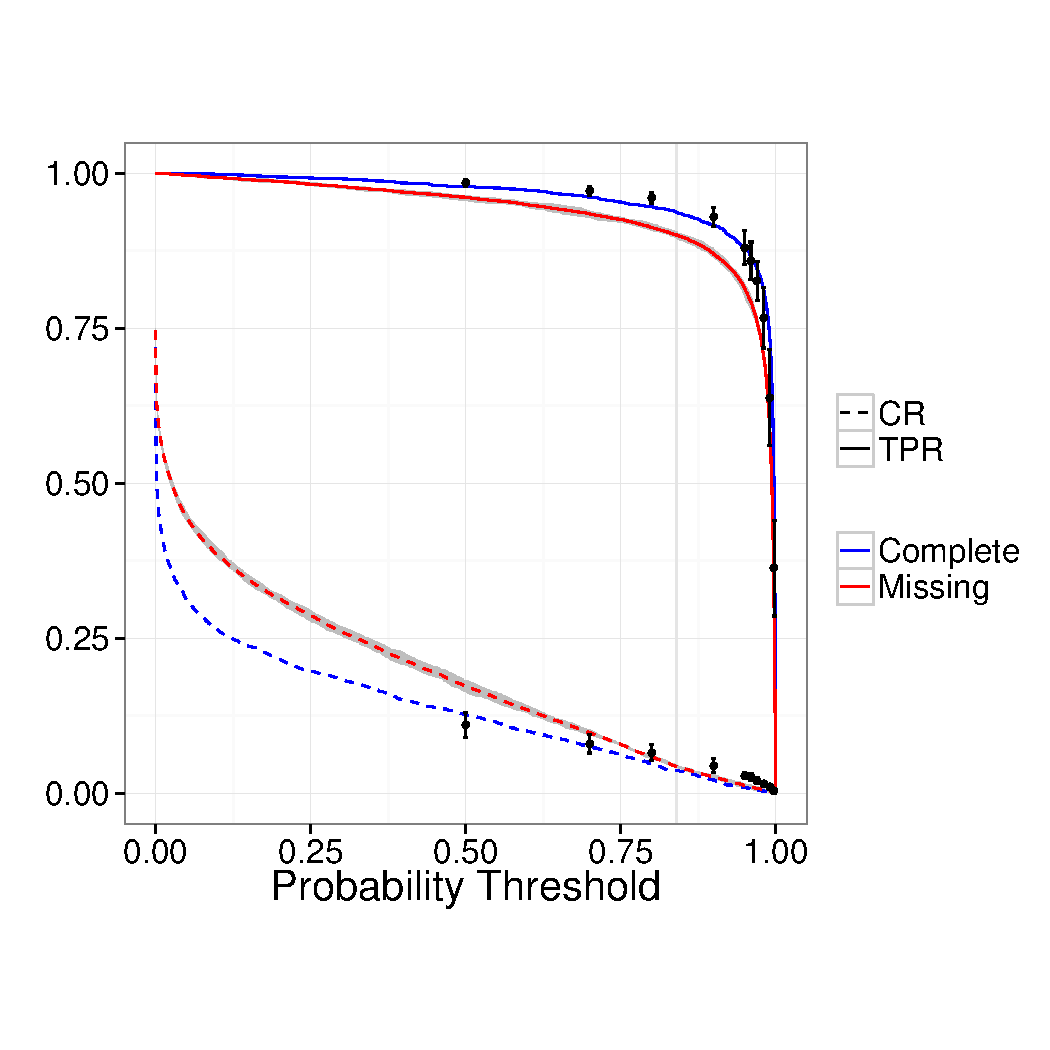
\includegraphics{background/Figures/FTPRvsSarro.pdf}}
\caption{The mean \gls{tpr} (solid line) and \gls{cr} (dashed line) resulting from five synthetic data sets including objects with missing entries (red lines). Also the \gls{tpr} and \gls{cr} resulting from a synthetic data set comprising only objects with fully observed vectors (blue lines). The shaded regions (grey) show the uncertainties computed from the five synthetic data sets. The black dots show the \gls{tpr} and \gls{cr} reported by \citet{Sarro2014} for their model. See text for warnings on this comparison. Reproduced from Figure 3 of \citet{Olivares2017},\textit{\usebibentry{Olivares2017}{Title}}, \usebibentry{Olivares2017}{Journal}, Vol. \usebibentry{Olivares2017}{Volume}.}
\label{fig:TPR-CR}
\end{center}
\end{figure}

\begin{figure}[ht!]
\begin{center}
\resizebox{0.8\textwidth}{!}{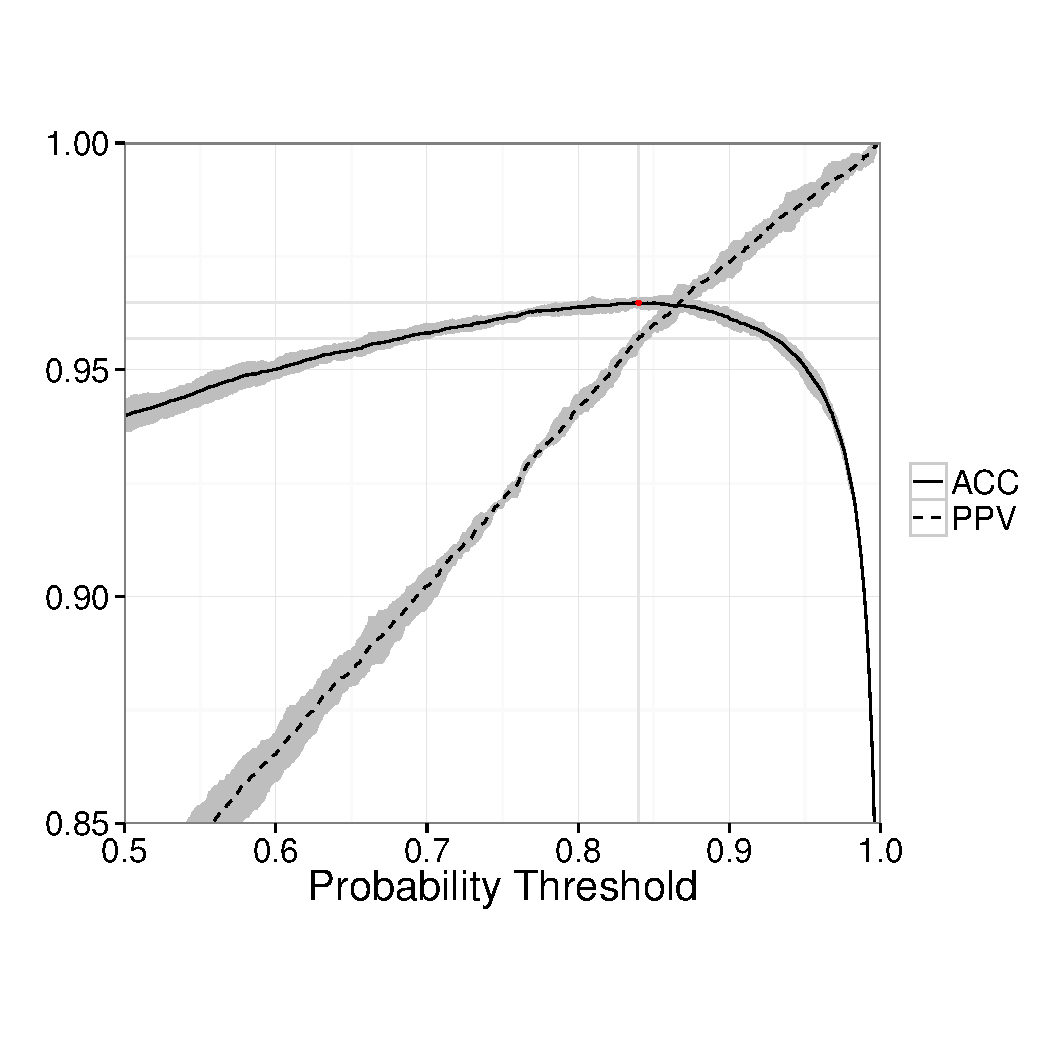
\includegraphics{background/Figures/PrecisionAccuracy.pdf}}
\caption{Mean accuracy (\gls{acc}, solid line) and precision (\gls{ppv}, dashed line) of the classifier as a function of probability threshold. The shaded regions shows the uncertainties computed from the five synthetic data sets. The higher accuracy is obtained at $p_t=0.84$ (red dot). Reproduced from Figure 3 of \citet{Olivares2017},\textit{\usebibentry{Olivares2017}{Title}}, \usebibentry{Olivares2017}{Journal}, Vol. \usebibentry{Olivares2017}{Volume}.}
\label{fig:ACC}
\end{center}
\end{figure}

We further investigate the impact that objects with missing value have on our methodology. In specific, I analyse possible biases introduced by these objects. To do this, I compare the membership probabilities inferred by the \gls{bhm} on:  i) the synthetic data set with fully observed objects (i.e. not a single missing value), and ii) a synthetic data set, created from the previous one, but with some observables masked as missing (using the procedure previously described).

In Fig. \ref{figure:IncVsCom}, I compare the mode of the recovered membership probabilities. The horizontal axis contains the membership probabilities of the data set with fully observed objects (I call this case the complete one). The vertical axis shows the membership probabilities of the same objects but in which some entries were masked as missing (I call this case the Incomplete one). As can be seen from this figure, the missing values impact our results by spreading the membership probabilities. Ideally, we would like to recover membership probabilities following the line of slope one. This is the case of the majority of fully observed objects (red squares) in the data set containing objects with missing entries. The most striking deviations come from those objects with the $\gls{ci}$ masked as missing (enclosed in black). The \gls{bhm} methodology uses the \emph{true} $\gls{ci}$ to prescribe the \emph{true} photometry. Also, it uses the observed $\gls{ci}$ to constrain the marginalisation integral of the \emph{true} $\gls{ci}$. Thus, as expected, a missing $\gls{ci}$ produces a spread in the membership probability.

The objects with a missing $\gls{ci}$ show two different behaviours. In one hand, the incomplete case (data set with missing values) overestimates the membership probabilities, while in the other case, it underestimate them. The former case is observed in the vertical stripe with $P \sim 0$ in the complete case, while the later case corresponds to those in the combed area below the line of unit slope.  Objects in the former case increase the \gls{cr}, and their effect can be seen by the difference between red and blue dashed lines in the lower-left region of Fig. \ref{fig:TPR-CR}. On the other hand, the objects in the latter case diminish the \gls{tpr}, and their effect can also be seen by the difference between red and blue solid lines in the top-right region of Fig. \ref{fig:TPR-CR}. 

The increase in \gls{cr} reaches its maximum near probability zero in the horizontal axis (Complete case) and goes to zero at probability thresholds of $\sim 0.9$. Therefore, the impact this increased \gls{cr} has in our results is marginal. For example, at the optimal probability threshold $p_t=0.84$, the increase of \gls{cr} due to objects with missing entries represent only 1.8\%. This fraction corresponds to those objects inside the black box of Fig. \ref{figure:IncVsCom} (upper left corner). However, the objects in the second case, those that diminish the \gls{tpr}, represent the typical unavoidable loss of members due to their missing entries. These amount to a 4\% loss in the \gls{tpr}, at the optimal probability threshold, $p_t=0.84$.


The bias introduced in the recovered membership probabilities due to objects with missing value entries, can be quantified using the root-mean-square (rms) of the difference between the means of the two recovered membership probabilities (Complete and Incomplete cases). The total rms is 0.12. On the one hand, fully observed objects in both data sets (Complete and Incomplete cases) have a rms of only 0.02. On the other hand, objects with missing entries, excluding those with missing $\gls{ci}$, have a rms of 0.08. The rms of objects lacking the $\gls{ci}$ is 0.14. The previous effects show an overall agreement between results on data sets with and without objects with missing entries. Nonetheless, care must be taken when dealing with individual membership probabilities. An object with a missing value in the $Y,J,H$ and $K_s$ may have a diminished membership probability (with a rms of 0.08), while an object with a missing $\gls{ci}$ may show an increased membership probability (with a rms of 0.14).  


However, as have been mentioned before, the methodology described in this work aims at the statistical distributions of the cluster population. The individual membership probabilities are just a useful by product. The methodology develop here, though, works by ensuring that each object contributes to the posterior distribution of the parameters modelling the cluster population, proportionally to its cluster membership probability. In this sense our results are free of any possible bias introduced by cuts in the membership probability. Nevertheless, there is still contamination. In particular, that arising from objects with missing entries. This contamination in the statistical distributions that we aim to obtain must be quantified. To do this, I compute the expected value of the \gls{cr} found in this section. It is $\langle \gls{cr} \rangle=5.8\pm 0.2$\%. In this expected value, each \gls{cr} contributes proportionally to the probability threshold at which it is measured. Since the vast contribution to this \gls{cr} coms from probability thresholds below 0.2 (see Fig. \ref{fig:TPR-CR}), the expected value of the \gls{cr} remains low. 

\begin{figure}[!htp]
\begin{center}
\resizebox{0.8\textwidth}{!}{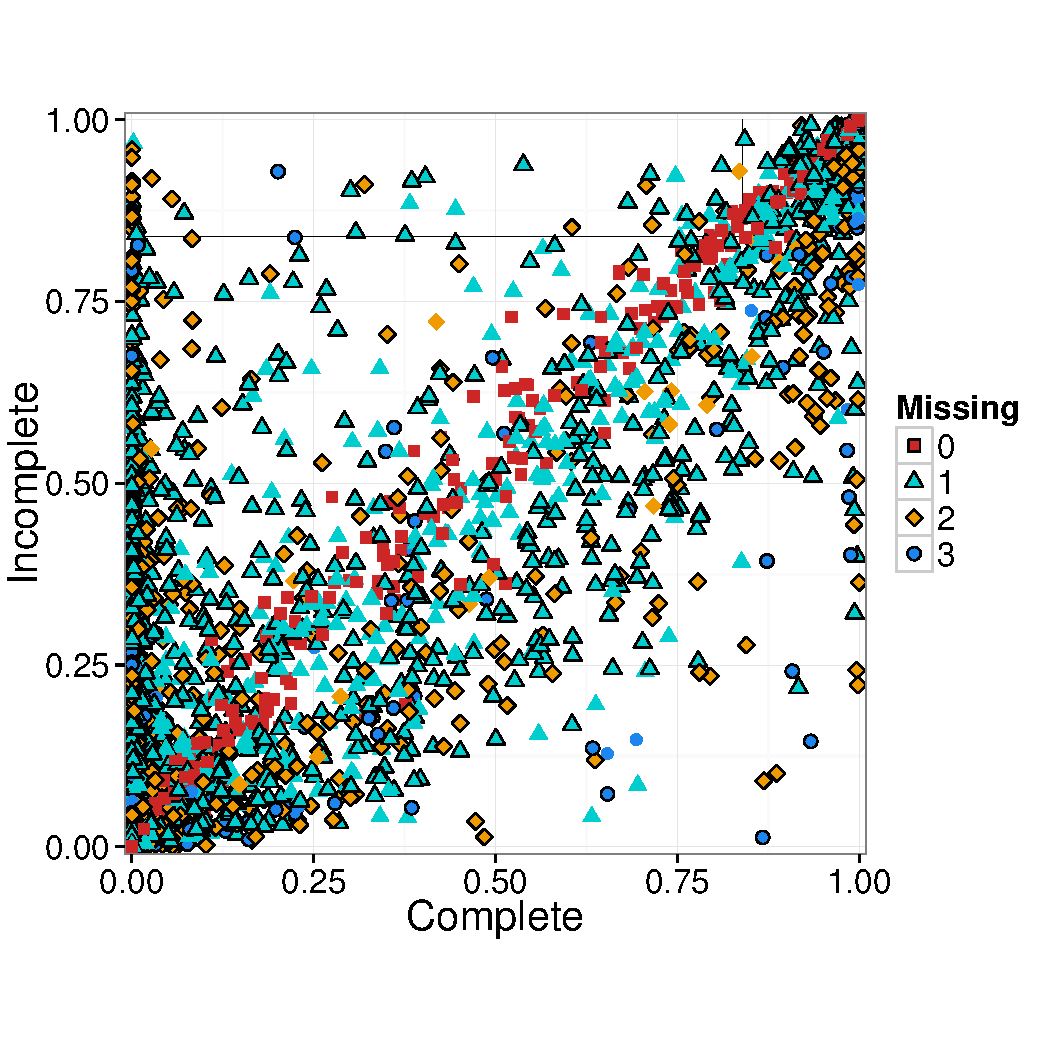
\includegraphics[page=1]{background/Figures/Probabilities.pdf}}
\caption{Comparison between the cluster membership probabilities recovered from the synthetic data set with objects having missing value entries (vertical axis, labeled Incomplete), and, the synthetic data set with fully observed objects (horizontal axis, labeled Complete). The colour and shape indicate the amount of missing entries. The symbols enclosed in black indicate a missing $\gls{ci}$. The top left box contains objects considered as contaminants due to missing values at the probability threshold $p_t=0.84$. Reproduced from Figure 4 of \citet{Olivares2017},\textit{\usebibentry{Olivares2017}{Title}}, \usebibentry{Olivares2017}{Journal}, Vol. \usebibentry{Olivares2017}{Volume}.}
\label{figure:IncVsCom}
\end{center}
\end{figure}

In statistical science, in machine learning particularly, is sometimes useful to analyse the performance of a binary classifier by means of the \glsfirst{roc} space. It is a visual diagnostic of the ability of the classifier to perform its job. The \gls{roc} space plots the \gls{tpr} as a function of the \gls{fpr}. A perfect classifier would be that in which the \gls{tpr}=1 and the \gls{fpr}=0. On the other hand, a random classifier, which will assign the class with a random probability (e.g. flipping a coin),  would be that with \gls{tpr}=\gls{fpr}=0.5. Such classifier lays in the line of slope one in the \gls{roc} space.

As an example, for one of the five synthetic data sets,  I classified objects with a binary random classifier with prior probabilities as those given by the fraction of field and cluster members (0.8 and 0.2, respectively, notice that the synthetic data sets have only $10^4$ objects). This is given by a binomial distribution with probability of success equal to 0.2. In ten random realisations of this classification, the \gls{tpr}=\gls{fpr}=0.5. In addition, the \gls{ppv} and \gls{cr} of such random classifier are $0.074\pm 0.003$ and $0.925\pm0.003$, respectively.

Furthermore, if the classifier returns a continuous random variable which then is used to do the classification, like the probability returned by the \gls{bhm}, instead of having a single point in the \gls{roc} space, the classifier produces a curve. The \gls{roc} curve of a perfect classifier will pass trough the point \gls{tpr}=1 and the \gls{fpr}=0, for a given classification threshold. The quantitative diagnostic for this kind of binary classifier is the \gls{auc} \gls{roc}. As its name indicate, the \gls{auc} is the integral of the \gls{roc} curve. Thus the closer the \gls{auc} is to one, the better the classifier is. In Fig. \ref{fig:ROC}, I show the \gls{roc} curve for our classifier when applied over synthetic data containing objects with missing entries. This \gls{roc} curve correspond to one of the five synthetic realisations described throughout this section. As can bee seen from this Figure our classifier does an excellent job, with an \gls{auc}=0.992.

\begin{figure}[!htp]
\begin{center}
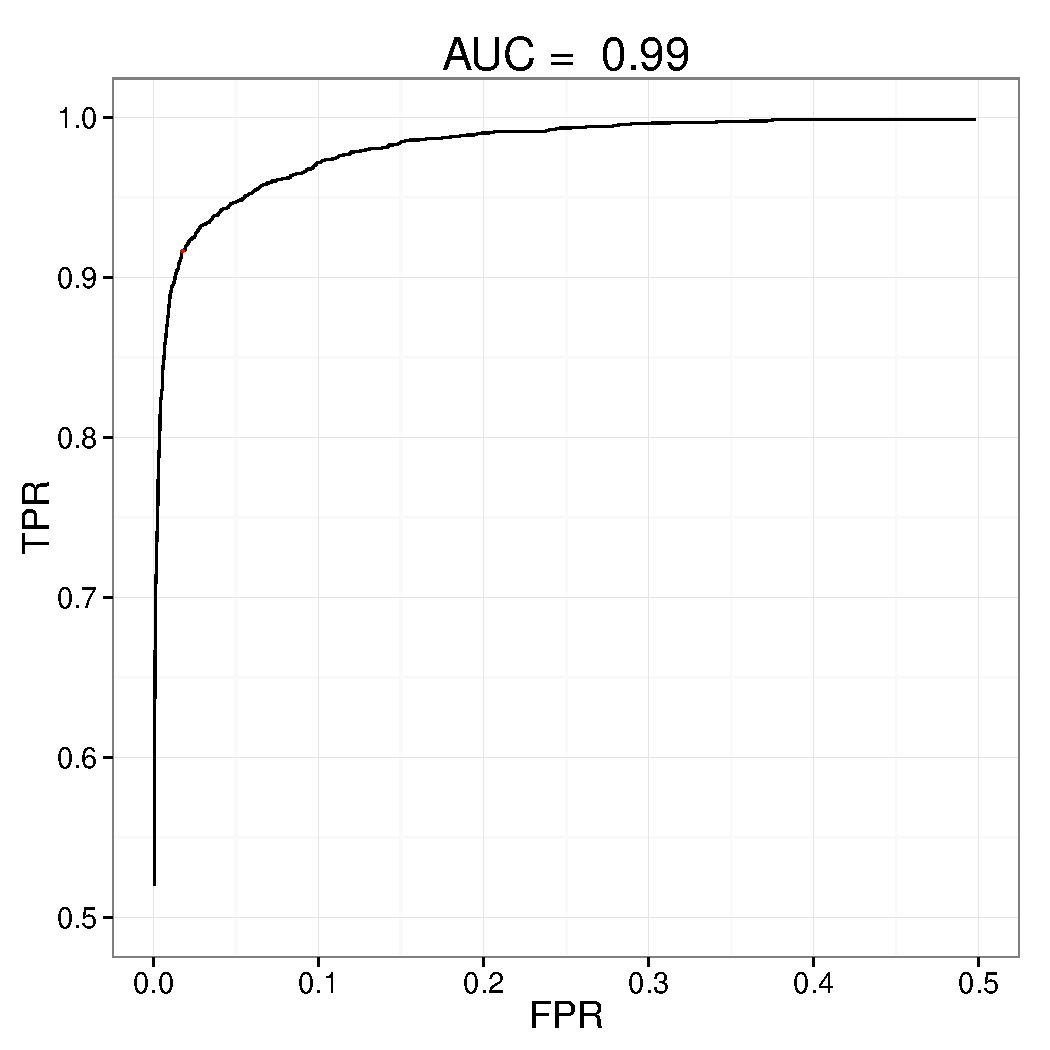
\includegraphics[page=1,width=0.8\textwidth]{background/Figures/ROC.pdf}
\caption{\gls{roc} curve of the \gls{bhm} by-product classifier when applied on the synthetic data set containing objects with missing entries. As can be seen, the \gls{auc}=0.992 diagnose it as an excellent classifier.}
\label{fig:ROC}
\end{center}
\end{figure}

 
\section{Comparison with the literature}
\label{sect:memberscomparison}

In the following, I will I compare the cluster membership probabilities recovered by the \gls{bhm} methodology, after applying it to the real \gls{rdr2}, with three sources from the literature: \citet{Stauffer2007}, \citet{Bouy2015} and \citet{Rebull2016}.

In the following I will refer to the \glsfirst{hmps} as those objects in the \gls{rdr2} from which the \gls{bhm} returns a membership probability distribution with a 84th percentile larger than the optimal probability threshold of 0.84 determined in the previous Section. The 84th percentile ensures that the uncertainty is taken into account. Figure \ref{fig:CsBs_members} shows the proper motions and $K_s$ vs \gls{ci} \glspl{cmd} of the \gls{hmps} of candidate members classified as single stars ($\langle p_{EMB} \rangle < 0.5$), and  \gls{emb} ($\langle p_{EMB} \rangle \geq 0.5$). In a similar way, Fig. \ref{fig:CsBs_members2} shows the $K_s$ vs $J-K_s$ \glspl{cmd} of the \gls{hmps} of candidate members.

\begin{figure}[ht!]
    \centering
    \begin{subfigure}[t]{0.45\textwidth}
       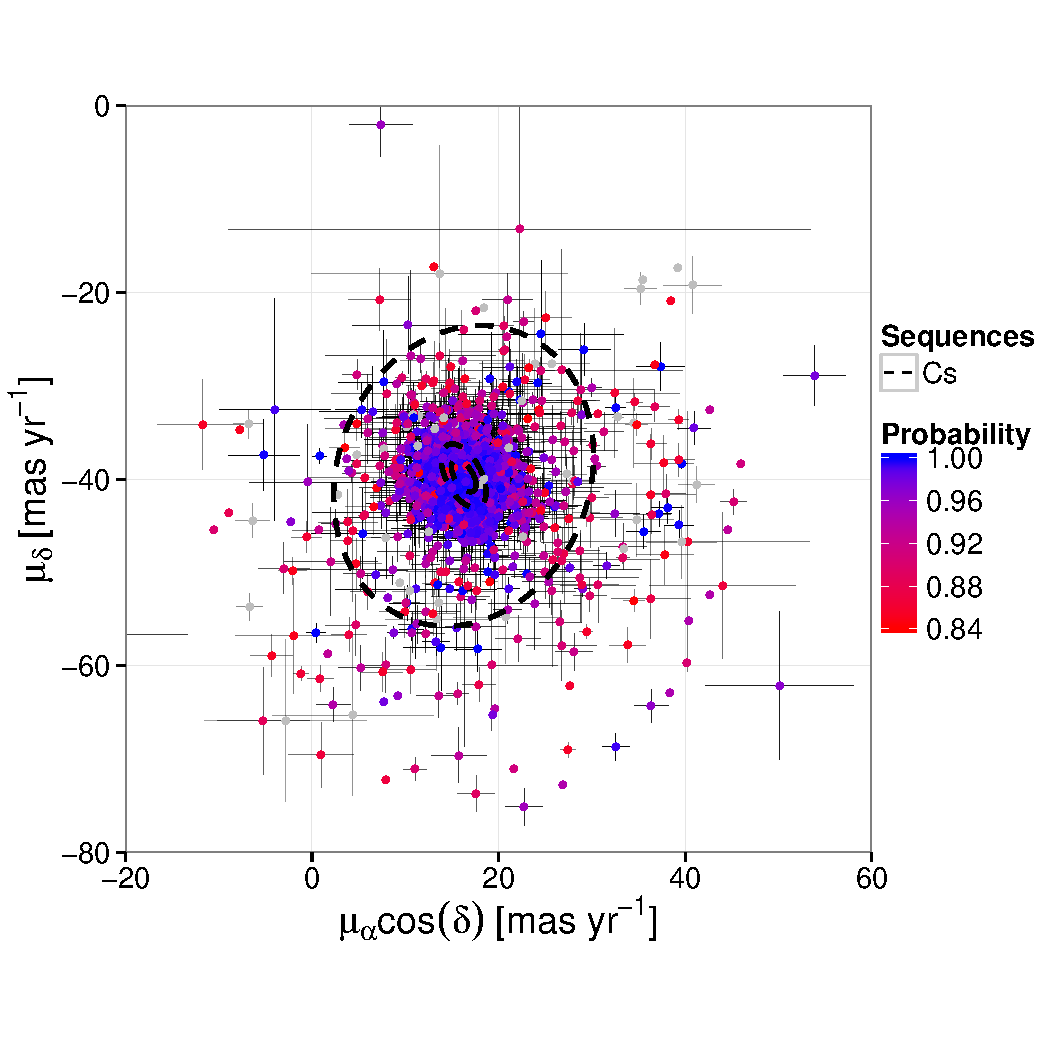
\includegraphics[page=1,width=\textwidth]{background/Figures/BHM/Cs_members.pdf}
    \end{subfigure}
    \begin{subfigure}[t]{0.45\textwidth}
     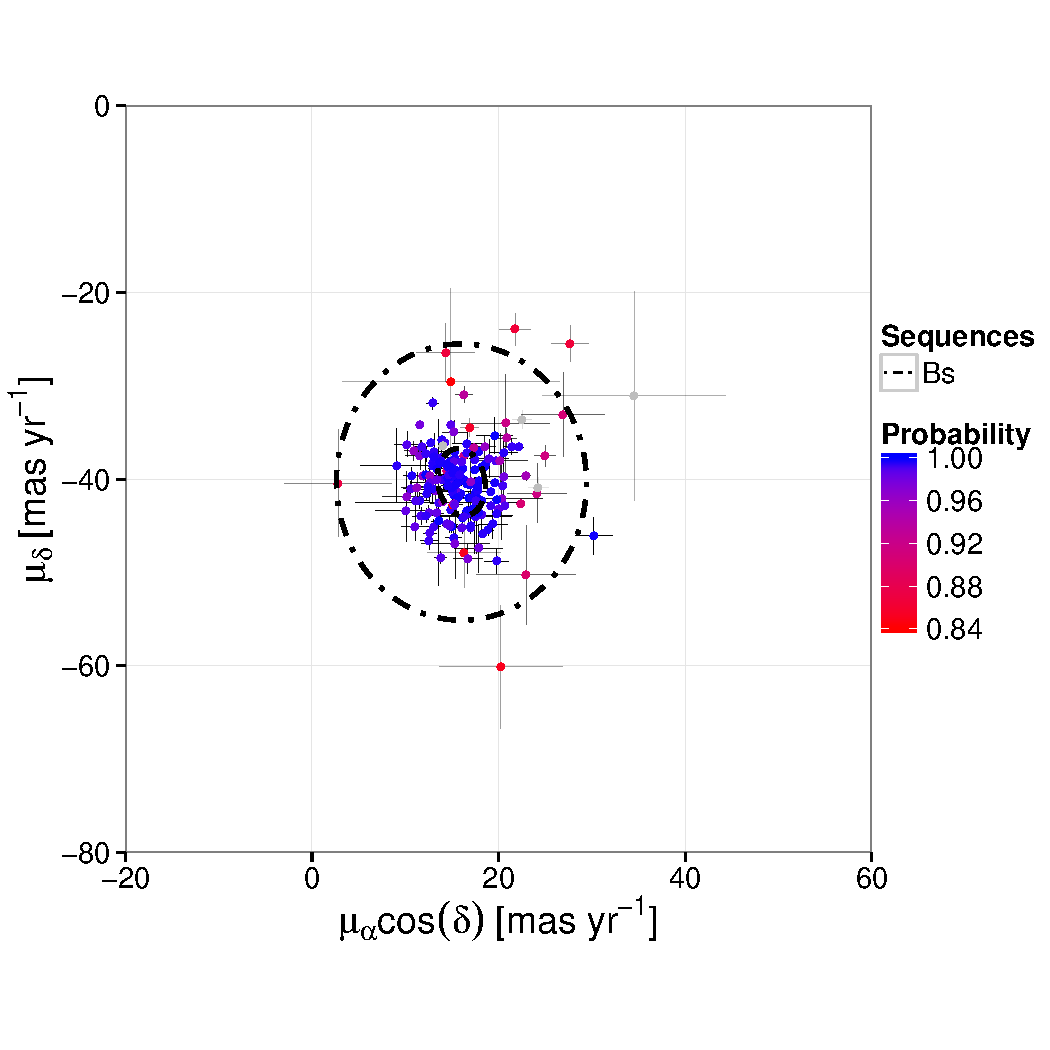
\includegraphics[page=1,width=\textwidth]{background/Figures/BHM/Bs_members.pdf}
    \end{subfigure}
    \begin{subfigure}[t]{0.45\textwidth}
       \includegraphics[page=7,width=\textwidth]{background/Figures/BHM/Cs_members.pdf}
    \end{subfigure}
    \begin{subfigure}[t]{0.45\textwidth}
     \includegraphics[page=7,width=\textwidth]{background/Figures/BHM/Bs_members.pdf}
    \end{subfigure}
\caption{Proper motions (top panels), and $K_s$ vs $i-K_s$ \glspl{cmd} (bottom panels)  of the \gls{hmps} of candidate members. The left panels show objects classified as single stars (with $\langle p_{EMB} \rangle < 0.5$), while the right panels those classified as \gls{emb} (with $\langle p_{EMB} \rangle \geq 0.5$). The colour code shows the mode of the individual cluster membership probabilities. Objects with $P_{84\%}> 0.84$ but mode lower than 0.84 are shown as grey dots. Also shown the mode of the parameters posterior distribution for single stars (Cs, dashed lines) and \gls{emb} (Bs, dot dashed lines).}
\label{fig:CsBs_members}
\end{figure}

\begin{figure}[ht!]
    \centering
  \begin{subfigure}[t]{0.45\textwidth}
  \includegraphics[page=9,width=\textwidth]{background/Figures/BHM/Cs_members.pdf}
  \end{subfigure}
    \begin{subfigure}[t]{0.45\textwidth}
     \includegraphics[page=9,width=\textwidth]{background/Figures/BHM/Bs_members.pdf}
    \end{subfigure}
\caption{$K_s$ vs $J-K_s$ \glspl{cmd} of the \gls{hmps} of candidate members. The left panel shows objects classified as single stars (with $\langle p_{EMB} \rangle < 0.5$), while the right panels those classified as \gls{emb}. Captions as in Fig. \ref{fig:CsBs_members}.}
\label{fig:CsBs_members2}
\end{figure}

Since the \gls{rdr2} is contained in the data set used by \citet{Bouy2015}, the comparison in this case can be extended not just to the common candidate members, but to all objects in the \gls{rdr2}. Furthermore, after applying the learned BHM to the entire \gls{ddr2} we found no newer members, which confirms our original assumption of an almost negligible probability of leaving a cluster member out of the \gls{rdr2}. Since no members are found outside the \gls{rdr2}, in the following the comparison between \citet{Bouy2015} membership probabilities and those estimated here is done based on the \gls{rdr2}.
 
 However, the comparison with \citet{Stauffer2007}, and \citet{Rebull2016} can only be done in terms of the candidate members in common. Since \citet{Rebull2016} obtain their list of candidates based on photometric variability, and this observable is not present in our set of observables, this comparison represent an important source of external validation. 


\subsection{Candidate members from \citet{Stauffer2007}}

\citet{Stauffer2007} published two list of candidate members. The first one contains 1417 objects compiled from the literature (see Table 2 of the mentioned work). These objects were classified as candidate members by several authors. As \citet{Stauffer2007} mention, this list is inhomogeneous, incomplete and certainly includes non-members. I refer to this list as \gls{st1}. Their second list contains 55 candidate members (see Table 5 of the mentioned work). \citet{Stauffer2007} found these members using infrared photometry and proper motions. I refer to this list as \gls{st2}.

Cross matching (at CDS\footnote{ Using the service http://cdsxmatch.u-strasbg.fr/xmatch}, within 1 arcsec radius) the previous two lists with the \gls{ddr2} catalogue \citep{Bouy2015}, I find that only 1384 and 54 of the \gls{st1} and \gls{st2} lists have a counter part in the \gls{ddr2} catalogue, respectively. 

Concerning our list of candidate members, after cross matching it with the two lists of \citet{Stauffer2007}, \gls{st1} and \gls{st2}, I recover 1146 and 34 of the candidate members, respectively. Compared to the candidate members of \citet{Bouy2015}, our \gls{bhm} recovers 28 more candidate members in \gls{st1} and the same in \gls{st2}.

As mentioned before, the \gls{st1} list is an exhaustive compilation of Pleiades members. It contains objects that were classified, at some point in history, as Pleiades candidate members, even when their membership probability are as low as 0.1 \citep{Stauffer2007}. For this reason I will not analyse the details of 238 rejected objects of \gls{st1}. It suffices to show that these rejected objects lie far from the cluster photometric or proper motions loci, as shown in Fig. \ref{fig:ST1}.

On the other hand, from the 20 objects in \gls{st2} that are rejected by the \gls{bhm}, 18 of them lie below the cluster photometric sequence and far from the proper motion locus, see Fig. \ref{fig:ST2}. The remaining two (\gls{dance} IDs: J034552.57+235145.9 and J034543.47+233851.5), although have observed photometric vectors compatible with the clusters sequence, their proper motions still are far from the cluster centre (with $\mu_{\alpha}\cos(\delta)\sim 40\,\rm{mas\cdot yr^{-1}}$), see Fig. \ref{fig:ST2}.

\begin{figure}[ht!]
    \centering
    \begin{subfigure}[t]{0.45\textwidth}
    \centering
       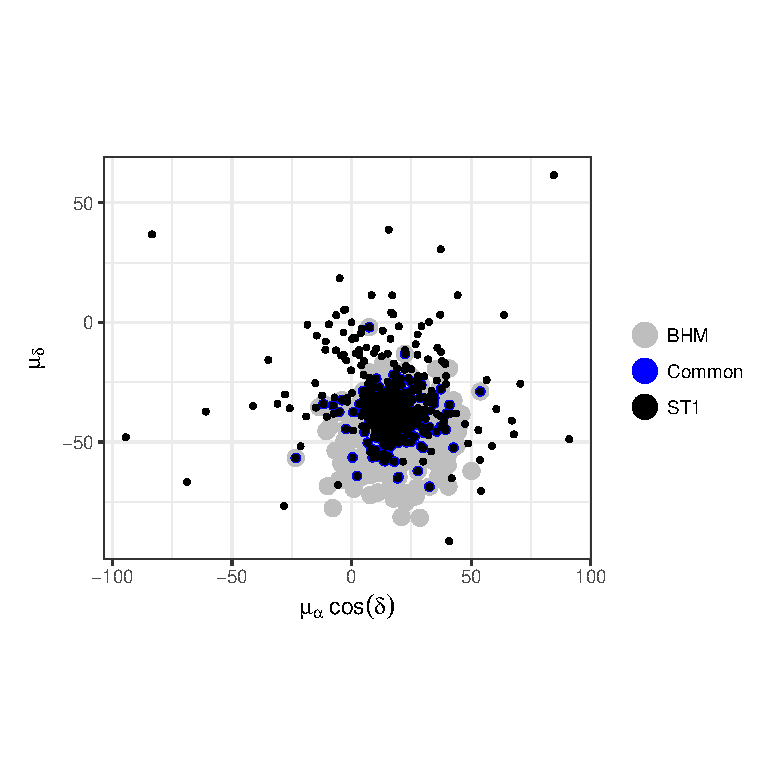
\includegraphics[width=\textwidth]{background/Figures/ST1_pm.eps}
        \caption{}
    \end{subfigure}
    \begin{subfigure}[t]{0.45\textwidth}
    \centering
     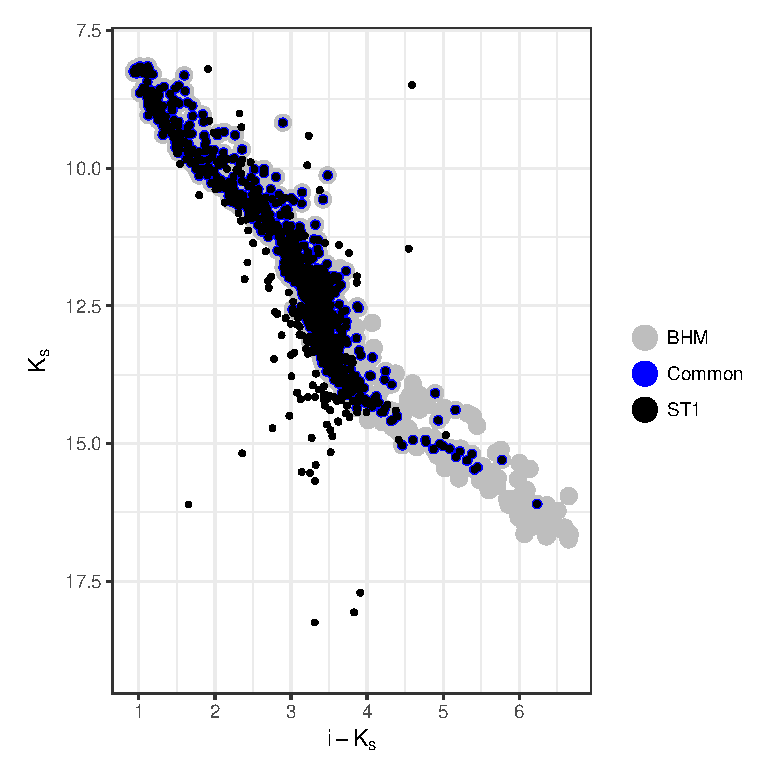
\includegraphics[width=\textwidth]{background/Figures/ST1_ph.eps}
        \caption{}
    \end{subfigure}
\caption{Proper motions (a) and $K$ vs $i-K$ \gls{cmd} (b) of the \gls{st1} candidate members in the \gls{ddr2} catalogue (black). Also shown, the objects classified as candidate members  in the \gls{bhm} (grey), and in both \gls{st1} and \gls{bhm} (blue).}
\label{fig:ST1}
\end{figure}

\begin{figure}[ht!]
    \centering
    \begin{subfigure}[t]{0.45\textwidth}
    \centering
       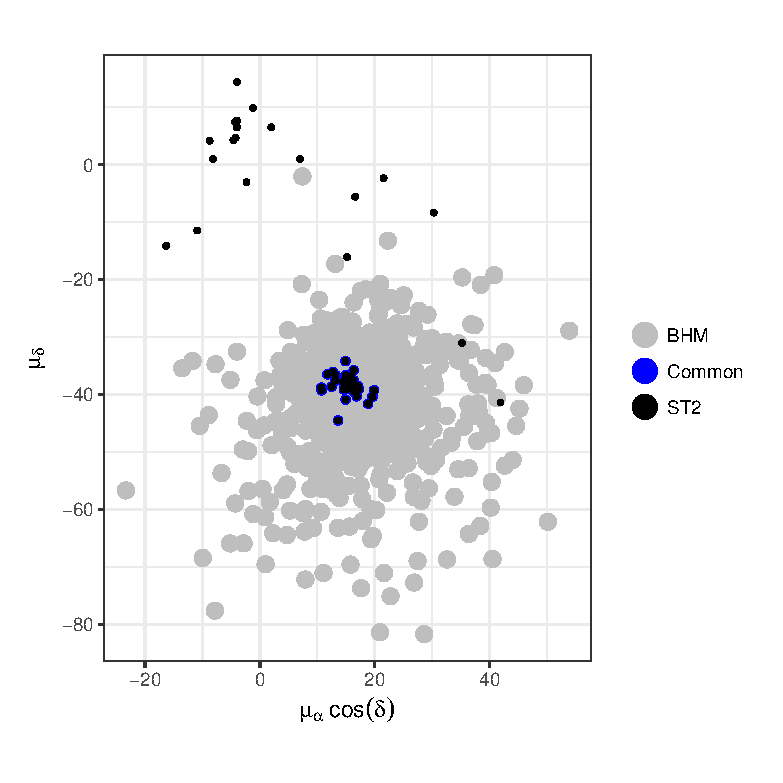
\includegraphics[width=\textwidth]{background/Figures/ST2_pm.eps}
    \end{subfigure}
    \begin{subfigure}[t]{0.45\textwidth}
    \centering
     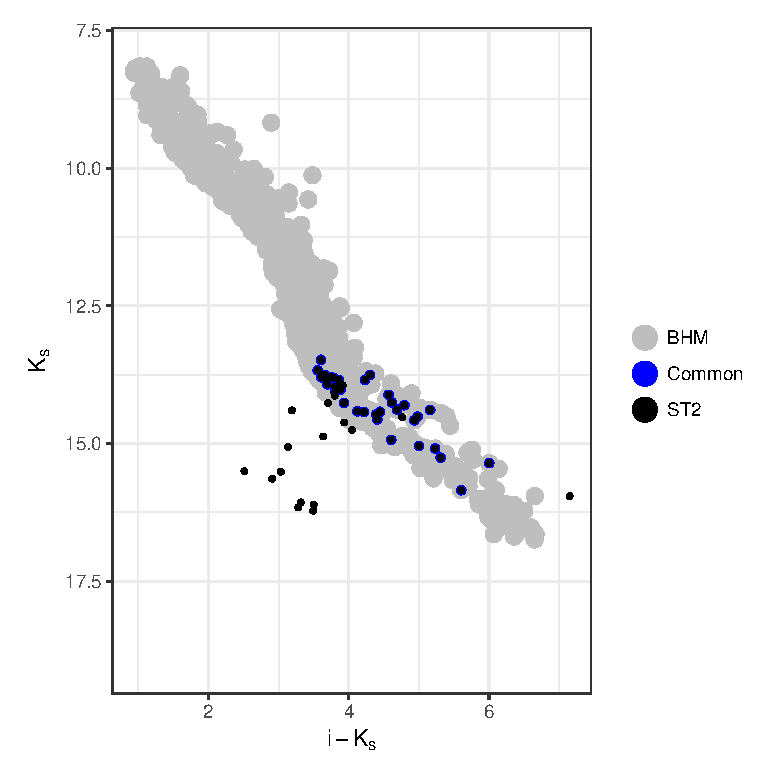
\includegraphics[width=\textwidth]{background/Figures/ST2_ph.eps}
        \caption{}
    \end{subfigure}
\caption{Proper motions (a) and $K$ vs $i-K$ \gls{cmd} (b) of the \gls{st2} candidate members in the \gls{ddr2} catalogue (black). Also shown, the objects classified as candidate members in the \gls{bhm} (grey), and in  both \gls{st2} and \gls{bhm} (blue).}
\label{fig:ST2}
\end{figure}

\subsection{Candidate members from \citet{Bouy2015}}
\label{sect:comparisonBouy}

The fact that the work of \citet{Bouy2015} and the present one use the same \gls{ddr2} data set (although our model is constructed with the \gls{rdr2}), allow me to directly compare the membership probabilities of both works. As mentioned before, this comparison can be extended to all objects in the data set and not just to the candidate members of the Pleiades cluster. Since \citet{Bouy2015} reported only an statistic of the membership probability distributions, to do a fair comparison, I summarise the membership probability distributions recovered by the \gls{bhm} with the mode.

Using the optimal probability threshold of 0.84 to classify the cluster members, we can see that, as shown by Fig. \ref{fig:BHMBouy}, both methodologies agree on the outstanding $99.6$\% of the classified objects. Concerning just the candidate members, the agreement is still high, $\sim 90\%$. In the following I discuss the 10\% discrepancies.

\begin{figure}[ht!]
\begin{center}
\resizebox{\textwidth}{!}{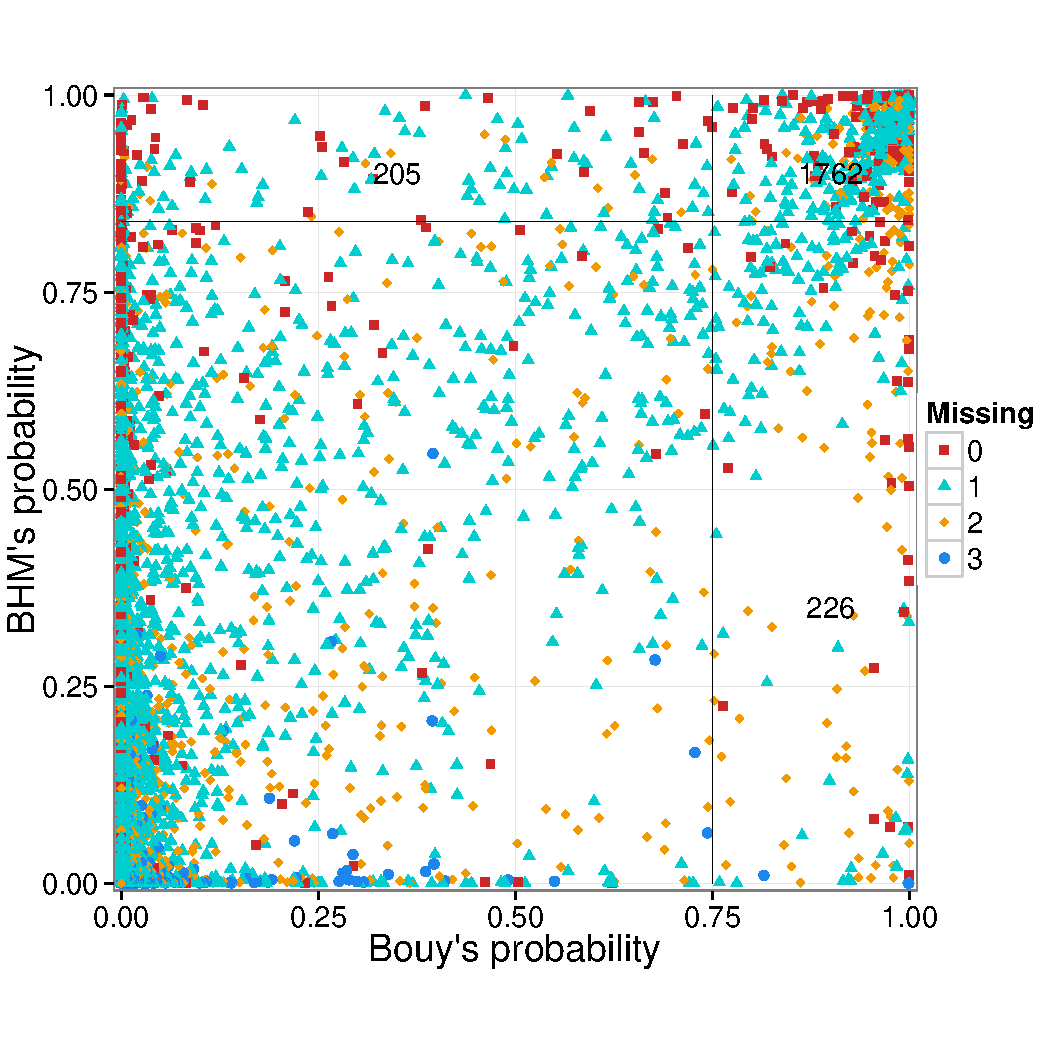
\includegraphics{background/Figures/BHM/BHMvsBouy.pdf}}
\caption{Mode of the membership probabilities recovered by the \gls{bhm} compared to those of \citet{Bouy2015}. The lines show the 0.75 and $p_t=0.84$ probability thresholds used in both works. The numbers indicate our new candidate members (top left), the ones we rejected (bottom right), and the common ones (top right). Reproduced from Figure 11 of \citet{Olivares2017},\textit{\usebibentry{Olivares2017}{Title}}, \usebibentry{Olivares2017}{Journal}, Vol. \usebibentry{Olivares2017}{Volume}.}
\label{fig:BHMBouy}
\end{center}
\end{figure}

The candidate members of \citet{Bouy2015} that the \gls{bhm} rejects, which I call the rejected ones, are shown in lower right box of Fig. \ref{fig:BHMBouy}. They amount to 12\% of the total number of candidate members recovered by \citet{Bouy2015}, and to 12.5\% of  candidate members recovered in the present work. The 12\% vale is larger, by 4.7\%, than the $7.3\pm1.4$\% of \gls{cr} reported by \citet{Sarro2014}, while the 12.5\% value is also larger, by 2.5\%, than the 10\% loss rate of the \gls{bhm} (the \gls{tpr}=90\% measured in Section \ref{sect:classifier}). These figures indicate that some true cluster members must be within the rejected objects, as expected from the \gls{tpr}=90\%.

Now, I analyse these objects with further detail. As it is shown in Figs. \ref{fig:rejecteds} and \ref{fig:rejectedsCOLORS}, the rejected objects have proper motions uncertainties with median $\tilde{\mu}_{\alpha},\tilde{\mu}_{\delta}=\{3.19,3.20\} \,\mathrm{mas\cdot yr^{-1}}$. This value is more than four times larger than that of the common candidate members (those objects classified as members by both works, see top right corner of Fig. \ref{fig:BHMBouy}), which have median $\tilde{\mu}_{\alpha},\tilde{\mu}_{\delta}=\{0.68,0.68\} \,\mathrm{mas\cdot yr^{-1}}$. Among the rejected ones, those with a relatively high membership probability occur mostly at the middle of the cluster photometric sequence (green squares of Fig. \ref{fig:rejectedsCOLORS}). On the other hand, those with lower membership probabilities occur at the bright and faint ends (blue and red triangles of Fig. \ref{fig:rejectedsCOLORS}, respectively). Furthermore, the proper motions uncertainties of the rejected objects at the bright, middle and faint ends of the cluster photometric sequence, have medians of $\tilde{\mu}_{\alpha},\tilde{\mu}_{\delta}=\{4.3,4.2\}  \,\mathrm{mas\cdot yr^{-1}}$, $\tilde{\mu}_{\alpha},\tilde{\mu}_{\delta}=\{2.4,2.4\}\,\mathrm{mas\cdot yr^{-1}}$ and $\tilde{\mu}_{\alpha},\tilde{\mu}_{\delta}=\{3.4,3.4\}\,\mathrm{mas\cdot yr^{-1}}$, respectively. These figures are approximately 6, 4 and 5 times larger, respectively, than those of the candidates in common. These large uncertainties produce a proportional spread of the cluster likelihood. This effect could reduce the membership probability of these objects.

 \begin{figure}[ht!]
\begin{center}
\resizebox{\textwidth}{!}{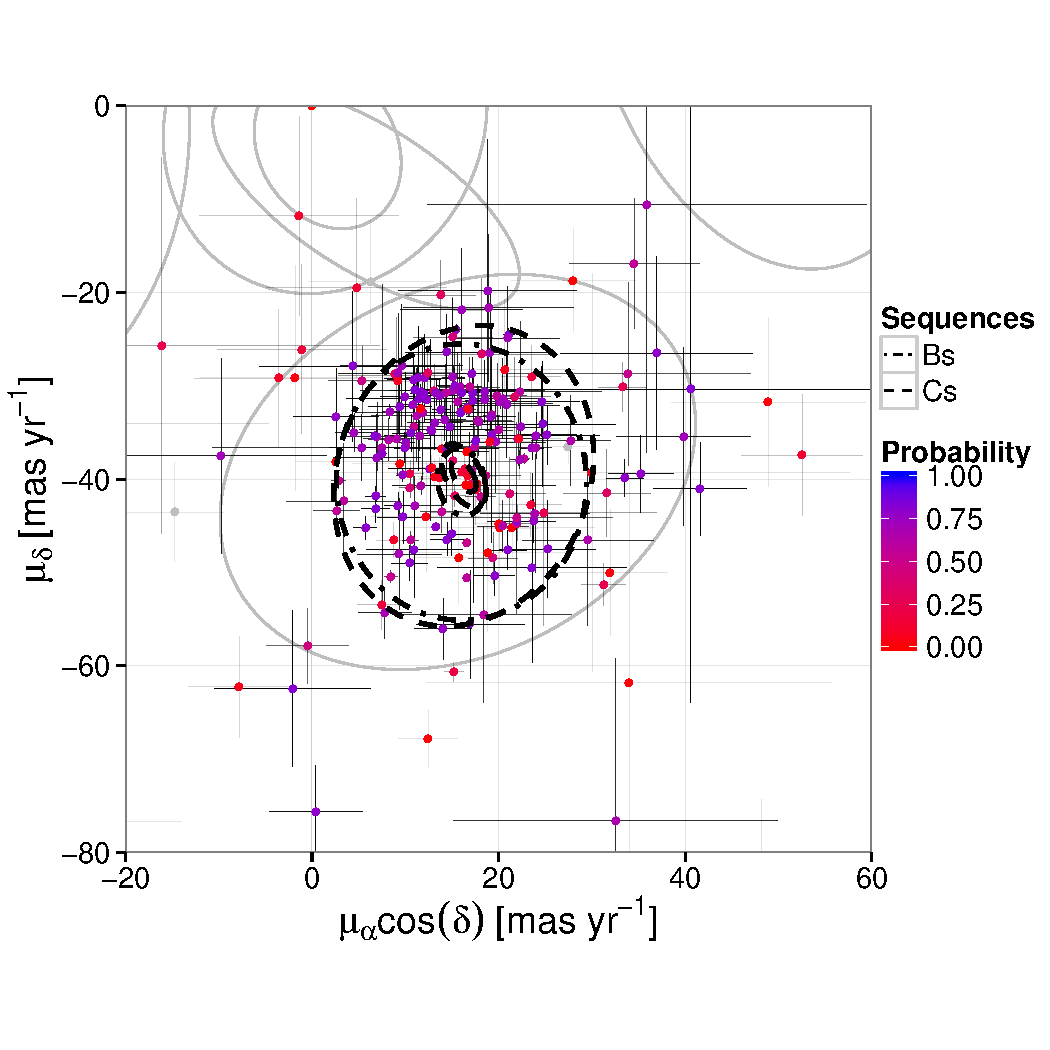
\includegraphics[page=1]{background/Figures/BHM/Rejecteds.pdf}\includegraphics[page=5]{background/Figures/Rejecteds.pdf}}
\caption{Proper motion (left) and $K_s$ vs. $i-K_s$ \gls{cmd} (right) showing the candidate members of \citet{Bouy2015} rejected by the \gls{bhm}. Reproduced from Figure 13 of \citet{Olivares2017},\textit{\usebibentry{Olivares2017}{Title}}, \usebibentry{Olivares2017}{Journal}, Vol. \usebibentry{Olivares2017}{Volume}.}
\label{fig:rejecteds}
\end{center}
\end{figure}

\begin{figure}[htbp]
\begin{center}
\resizebox{\hsize}{!}{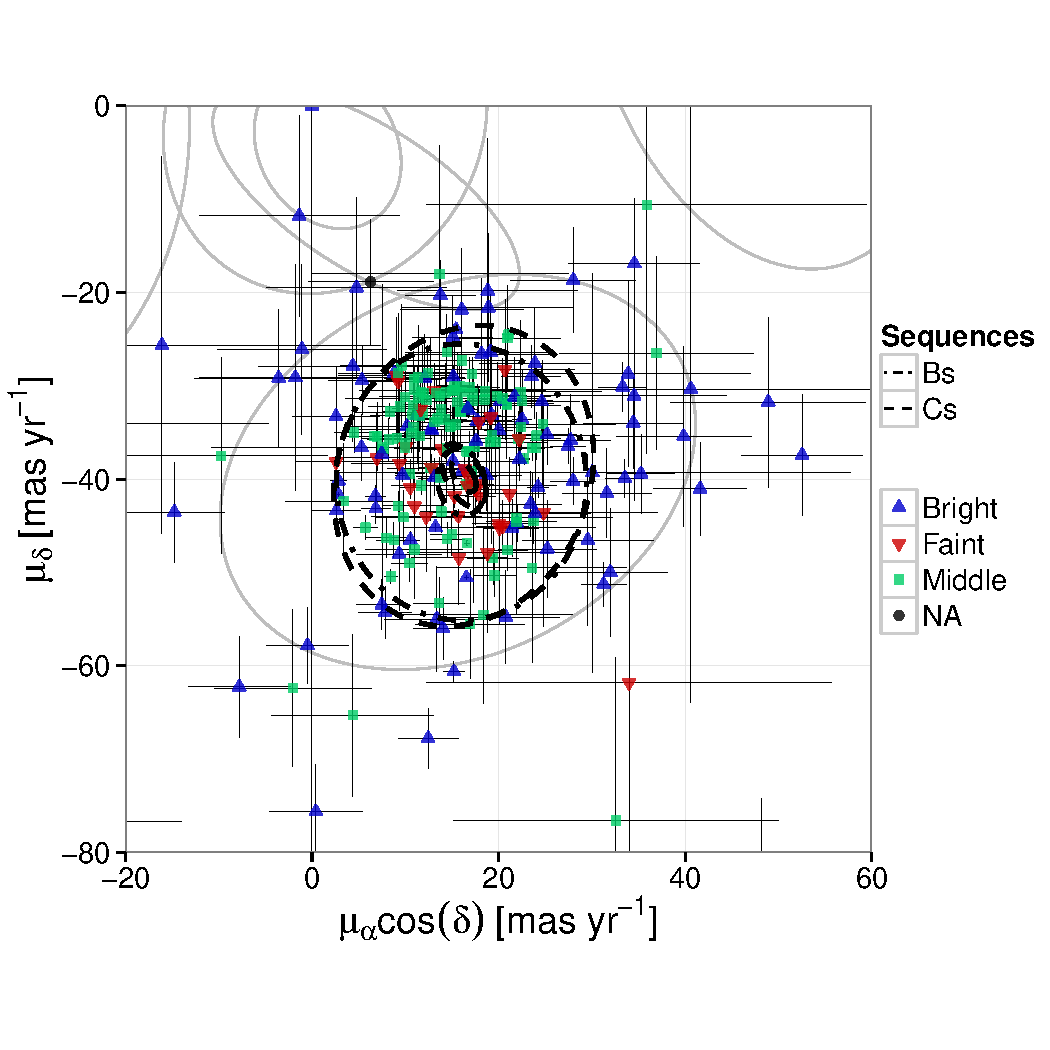
\includegraphics[page=1]{background/Figures/BHM/RejectedsCOLORS.pdf}\includegraphics[page=5]{background/Figures/RejectedsCOLORS.pdf}}
\caption{Proper motion (left) and $K_s$ vs. $i-K_s$ \gls{cmd} (right) showing the candidate members of \citet{Bouy2015} rejected by the \gls{bhm}. The colours and shapes are a proxy for their $K_s$ magnitude.Reproduced from Figure 14 of \citet{Olivares2017},\textit{\usebibentry{Olivares2017}{Title}}, \usebibentry{Olivares2017}{Journal}, Vol. \usebibentry{Olivares2017}{Volume}.}
\label{fig:rejectedsCOLORS}
\end{center}
\end{figure}

In addition to the large proper motion uncertainties of these objects, their membership probabilities are also affected by the different photometric cluster-to-field likelihood ratios in the \gls{bhm} and in \citet{Sarro2014} methodology, the one used by \citet{Bouy2015}.

Assuming that the field likelihoods of both models are the same, then the lower membership probabilities of the rejected objects result from the lower cluster likelihoods, which can be explained by the diverse ways in which both works model the spread of the cluster sequence. In \citet{Sarro2014} the latter is modelled as a multivariate normal with a covariance matrix estimated from objects in intervals of equal length along the cluster sequence (their so called $\lambda$). In addition, they mention that their methodology is sensitive to the observational uncertainties, thus their covariance matrices are overestimated. In summary, their method is sensitive to both the observational uncertainties and the number of objects along the cluster sequence. In the \gls{bhm} the spread of the cluster sequence is also multivariate normal but with covariance matrix that is: i) the true cluster sequence (i.e. the observational uncertainties are deconvolved), and ii) constant across the cluster sequence (i.e. independent of the number of sources in the length interval) and with a value inferred as the average spread (see Section \ref{subsect:cluster}).  Therefore, in \citet{Bouy2015} the spread of the cluster sequence compared to that of the \gls{bhm} is: a) overestimated in the faint and bright ends, where members are fewer and uncertainties larger, and b) underestimated in the central region (\gls{ci}=3.2) where members are copious and highly concentrated (see Figs. \ref{fig:CsBs_members} and \ref{fig:CMDs_results}). Thus, in the \gls{bhm} the the cluster likelihood of objects in cases a) and b) are both diminishes with respect to the cluster likelihood of \citet{Bouy2015}. For the objects in the first case (a), the cluster sequence is narrower, and thus their membership probability diminishes in proportion to their distance to the sequence. For objects in the second case (b),  the cluster sequence is wider and thus their cluster likelihood and membership probability diminishes. Both these effects are seen in Fig. \ref{fig:rejectedsJ_K}, where objects in the first case have membership probabilities below 0.5 (red dots), while objects latter case have membership probabilities near the classification threshold 0.84 (purple dots).

 \begin{figure}[ht!]
\begin{center}
\resizebox{\textwidth}{!}{\includegraphics[page=7]{background/Figures/BHM/Rejecteds.pdf}\includegraphics[page=7]{background/Figures/RejectedsCOLORS.pdf}}
\caption{$K_s$ vs. $J-K_s$ \glspl{cmd} showing the candidate members of \citet{Bouy2015} rejected by the \gls{bhm}. Captions in left and right panels are equivalent to those in Fig. \ref{fig:rejecteds} and \ref{fig:rejectedsCOLORS}, respectively.}
\label{fig:rejectedsJ_K}
\end{center}
\end{figure}

Assuming the alternative scenario in which the cluster likelihood of the \gls{bhm} and \citet{Bouy2015} is the same, the diminished membership probabilities of the rejected candidates \citet{Bouy2015} can be explained by the different ways in which the field likelihoods of both works are constructed. As explained in Section \ref{sect:current_methodologies}, the field likelihood in \citet{Sarro2014} methodology (the one used by \citet{Bouy2015}) is constructed only with fully observed objects (i.e. without missing values), which I called the \emph{naivety} assumption in Section \ref{sect:ignorability}. In that Section it is shown that such assumption leads to underestimate the field density in the bright and faint regions, and overestimate it in the middle region (see Fig \ref{fig:ignorable_and_naive}). Underestimating the field likelihood increases the cluster-to-field likelihood ratio and therefore the cluster membership probabilities. 

The previous phenomena acting together are responsible for the relatively lower \gls{bhm} membership probabilities of the rejected candidate members of \citet{Bouy2015}. A detailed comparison of the cluster and field likelihoods in both the \gls{bhm} and \citet{Bouy2015} models for each of the 226 objects lays beyond the objective of the present work. Nevertheless, these objects can not be discarded as potential true cluster members. As detailed in Section \ref{sect:classifier}, within these objects lays a fraction of the 10\% true cluster members below the 0.84 probability threshold. It is let to future works to disentangle which of these objects are true cluster members. 

On the other hand, the new candidates members found by the \gls{bhm}, shown in the upper left box of Fig. \ref{fig:BHMBouy}, amount to 10\% of the \citet{Bouy2015} candidate members. This figure is higher than the $\sim 3.5\%$ of missing rate (1-\gls{tpr}) reported by \citet{Sarro2014}. Also, these new candidates amount to 10\% of the \gls{bhm} recovered candidate members. This value is larger than the 4.3\% \gls{cr} reported in Section \ref{sect:classifier}. These two larger figures may indicate that some truly new discoveries may be within these list of new candidate members. In Figs. \ref{fig:newones} I show the proper motions and $K_s$ vs $i-K_s$ \gls{cmd} of these new candidates members.

The new candidate members have proper motions uncertainties whose median, $\tilde{\mu}_{\alpha},\tilde{\mu}_{\delta}=\{1.41,1.41\} \,\mathrm{mas\cdot yr^{-1}}$, is two times larger than those of the candidate members in common with \citet{Bouy2015}. Also, as shown by Fig. \ref{fig:newones}, the majority of the new candidate members, 166, have probabilities lower than 0.95, are located in a halo around the locus of the cluster proper motions, and on top of the cluster photometric sequence in the $K_s$ vs $i-K_s$ \gls{cmd}. On the contrary, the new candidate members with probabilities higher than 0.95, which are 39, lie in the centre of the cluster proper motions and fall above the cluster sequence in the $K_s$ vs $i-K_s$ \gls{cmd}. Thus, I hypothesise that: i) Objects whose photometry is compatible with the cluster sequence but are in the proper motions halo, have higher membership probabilities in our methodology due to the increased flexibility of the cluster proper motions model: it now has four gaussians instead of the two of \citet{Bouy2015}. And ii) objects near the centre of the cluster proper motions but located above the cluster photometric sequence sequence, are multiple systems \cite[probably triple systems which can amount to 4\% of the population][]{Duquennoy1991} with an increased membership probability due to our more flexible photometric model of the cluster and equal-mass binaries sequences.

 \begin{figure}[ht]
\begin{center}
\resizebox{\hsize}{!}{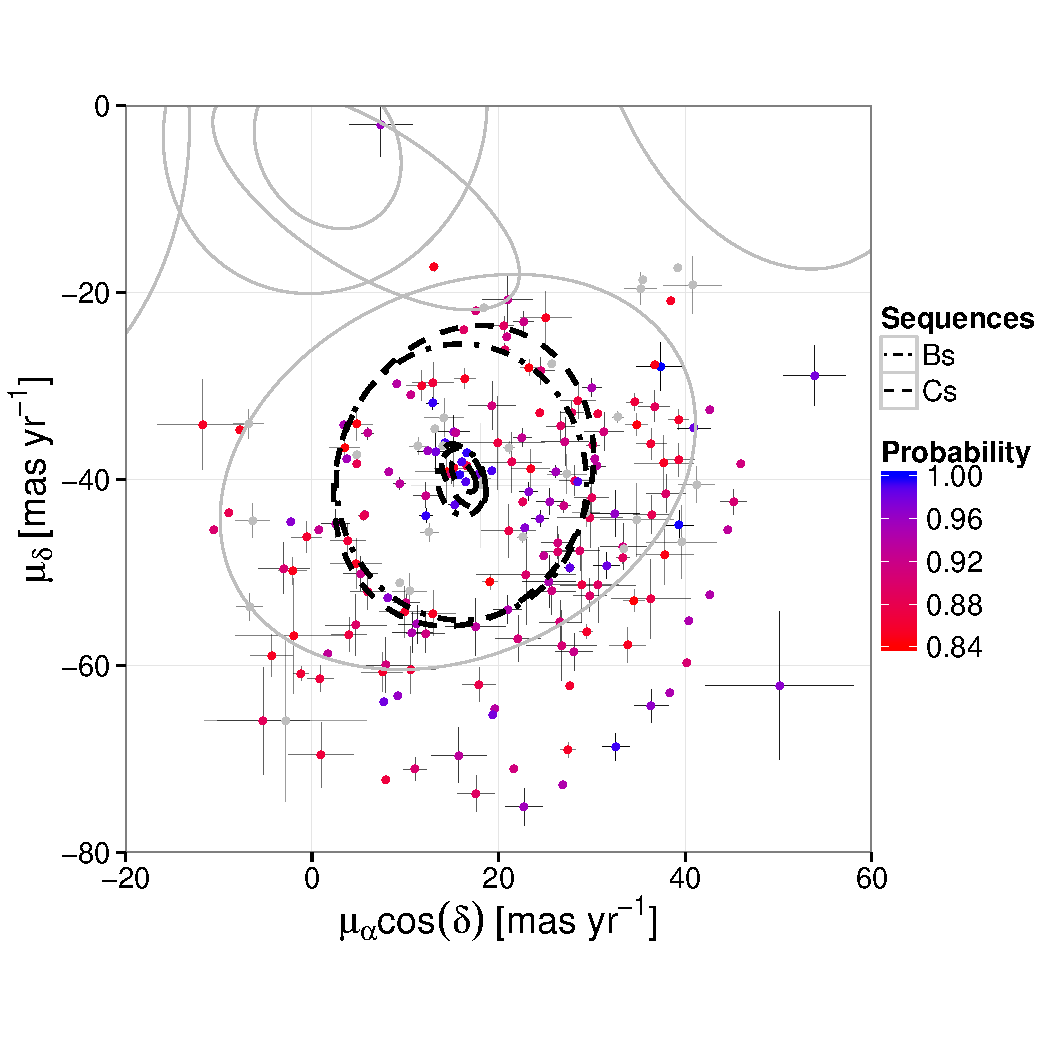
\includegraphics[page=1]{background/Figures/BHM/NewOnes.pdf}\includegraphics[page=5]{background/Figures/NewOnes.pdf}}
\caption{Proper motion (left) and $K_s$ vs. $i-K_s$ \gls{cmd} (right) showing the new candidate members found in this work. Reproduced from Figure 12 of \citet{Olivares2017},\textit{\usebibentry{Olivares2017}{Title}}, \usebibentry{Olivares2017}{Journal}, Vol. \usebibentry{Olivares2017}{Volume}.}
\label{fig:newones}
\end{center}
\end{figure}


Summarising, the discrepancies between the \gls{bhm} membership probabilities and those reported by \citet{Bouy2015} arise from subtle but important differences. The first difference is the treatment of object with missing entries. Although  \citet{Bouy2015} report membership probabilities for this kind of objects, their field and cluster models were constructed discarding them. As it is shown in Section \ref{sect:ignorability}, working with completely observed objects leads to a density which is in average more than three times more biased than one derived in this work. Although the field density derived in this work is also biased (see Section \ref{sect:ignorability}), including in our model objects with missing entries has two important consequences. First, the photometric model is more accurate than any other model that discards objects with missing entries (see Section  \ref{sect:ignorability}). This effect is important in the regions where these objects are more frequent. Second, the use of objects with missing entries in the construction of the cluster model allow us to include the information of good candidate members that were otherwise discarded a priori. 

In addition to the mentioned bias in the field density, I remind the reader of the bias present in the membership probability of objects with missing \gls{ci} (see Section \ref{sect:classifier}). In Fig. \ref{fig:BHMBouy}, the vertical stripe at $p_{Bouy} < 0.1$ and $p_{BHM} > 0.5$ there are 536 objects, from which the 80\% have missing entries, 76\% have a missing \gls{ci} and 4\% a missing band, and only 20\% have completely observed entries. While objects with missing \gls{ci} could be biased with an rms of 0.14, the completely observed ones are basically unbiased with an rms of 0.02. In Section   \ref{sect:classifier}, I stressed that particular care must be taken with the membership probabilities of objects with a missing \gls{ci}. However, the objects with completely observed entries laying within this stripe suggest that \citet{Bouy2015} methodology is too restrictive. Thus, the \gls{bhm} has a higher cluster model flexibility, which allows it to increase the membership probability of the previously discarded candidates.

\subsection{Candidate members from \citet{Rebull2016}}
\label{sect:comparisonRebull}

After cross matching (at CDS with a 0.5 arcsec radius) the list of candidate members from \citet{Rebull2016} (their Table 2, here after \gls{rt1}) with the  \gls{ddr2}, I find that 758 out of the 759 objects have a counter part in the \gls{ddr2} catalogue. The 91\% of these objects (690 of them) are candidate members in the \gls{bhm}. Under the assumption that the candidate members in \gls{rt1} are indeed true members, which may not be true, the ratio of recovered members is even better than the $\gls{tpr}=90\pm0.2\%$ reported in Section \ref{sect:classifier}. These objects are shown in Fig. \ref{fig:RT1}.

\begin{figure}[ht!]
    \centering
    \begin{subfigure}[t]{0.45\textwidth}
    \centering
       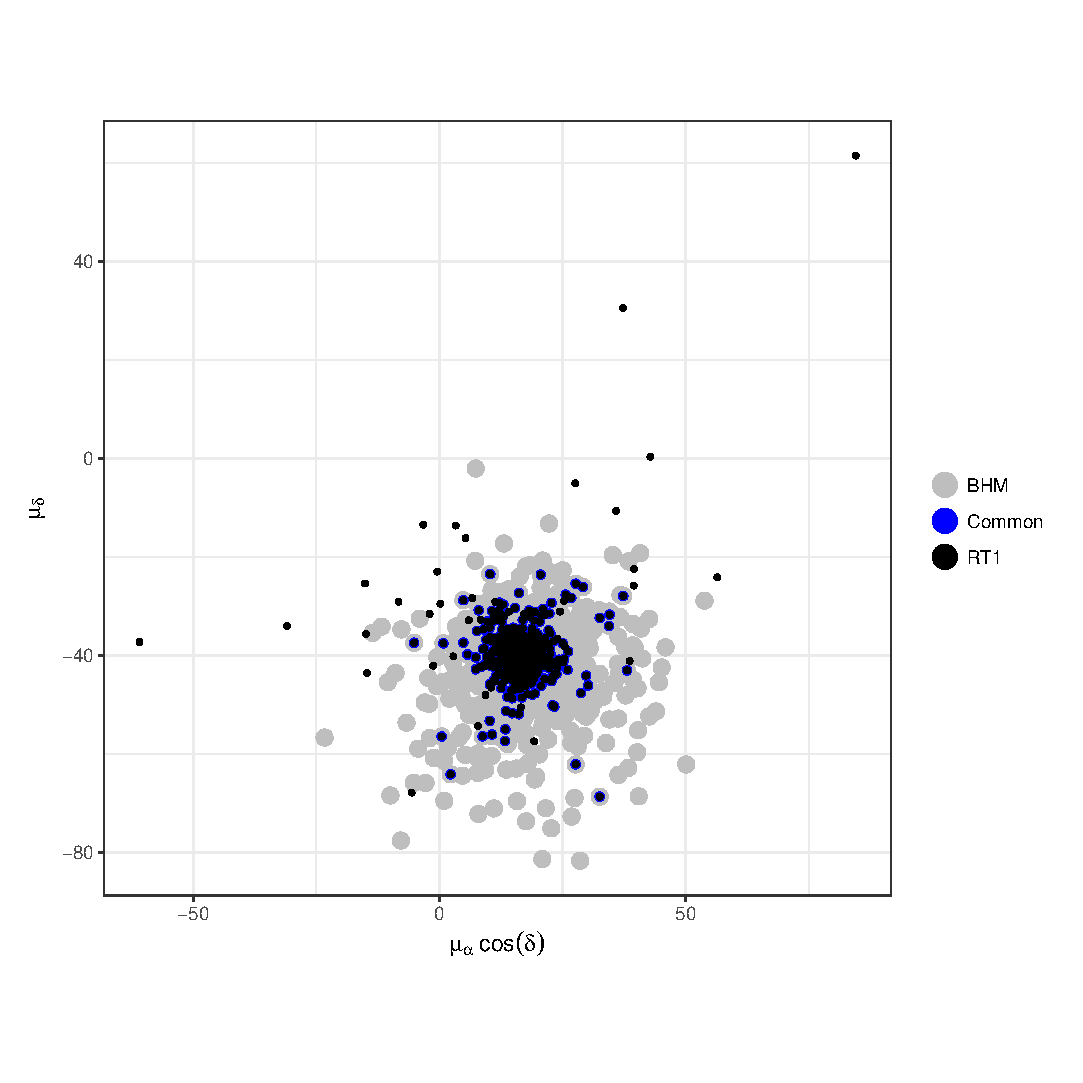
\includegraphics[width=\textwidth]{background/Figures/RT1_pm.eps}
        \caption{}
    \end{subfigure}
    \begin{subfigure}[t]{0.45\textwidth}
    \centering
     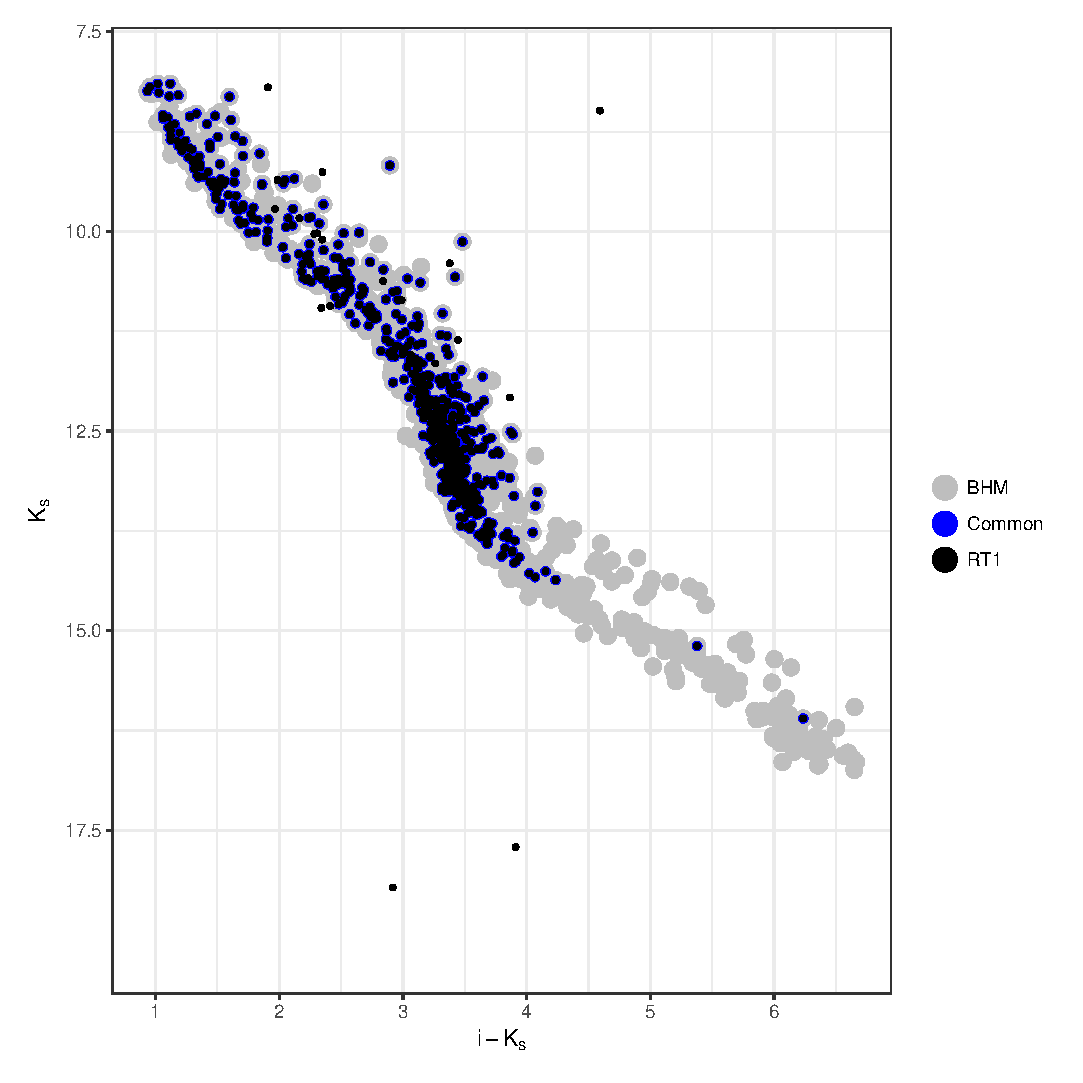
\includegraphics[width=\textwidth]{background/Figures/RT1_ph.eps}
        \caption{}
    \end{subfigure}
\caption{Proper motions (a) and $K$ vs $i-K$ \gls{cmd} (b) of the \gls{rt1} candidate members in the \gls{ddr2} catalogue (black). Also shown, the objects classified as candidate members  in the \gls{bhm} (grey), and in both \gls{rt1} and \gls{bhm} (blue).}
\label{fig:RT1}
\end{figure}

On the other hand, after cross matching (at CDS with a 0.5 arcsec radius)  the list of 154 objects that \citet{Rebull2016} classify as non-members (their Table 6, here after \gls{rt2}) with the \gls{ddr2}, I find that all these objects have a counter part on the \gls{ddr2}. The 21\% of objects in the \gls{rt2} list (33 of them) were classified as candidate members in the \gls{bhm}. This is a value five times larger than the \gls{cr} reported in Section \ref{sect:classifier} (\gls{cr}=4.3\%). However, we can not assume that the \gls{rt2} list comprises only non-members. First, this objects were at some point classified as members by other authors \cite[Appendix B of][]{Rebull2016}. Second, not all of these objects have periods \cite[only 20\% according to][]{Rebull2016}. From the 33 objects classified as candidate members by the \gls{bhm}, only nine of them have periods. It means that for the remaining 24 candidate members, these authors used other criteria to discard them as members. About their classification process, \citet{Rebull2016} say ``This process was qualitative in the sense that we weighted all of the information in a subjective manner. However, the process was also extensive, with each star considered individually and with all available information considered in detail. [...] we believe that in the great majority of cases we have made the right decision.'' In any case, the high rate of \gls{bhm} candidate members found in this \gls{rt2} list may indicate that either our contamination rate is underestimated or that the criteria used by \citet{Rebull2016} are too restrictive. As can be seen in Fig. \ref{fig:RT2}, these 33 objects have proper motions and photometric measurements consistent with those of the cluster. In order to clarify the status of these objects, further information is still needed.

\begin{figure}[ht!]
    \centering
    \begin{subfigure}[t]{0.45\textwidth}
    \centering
       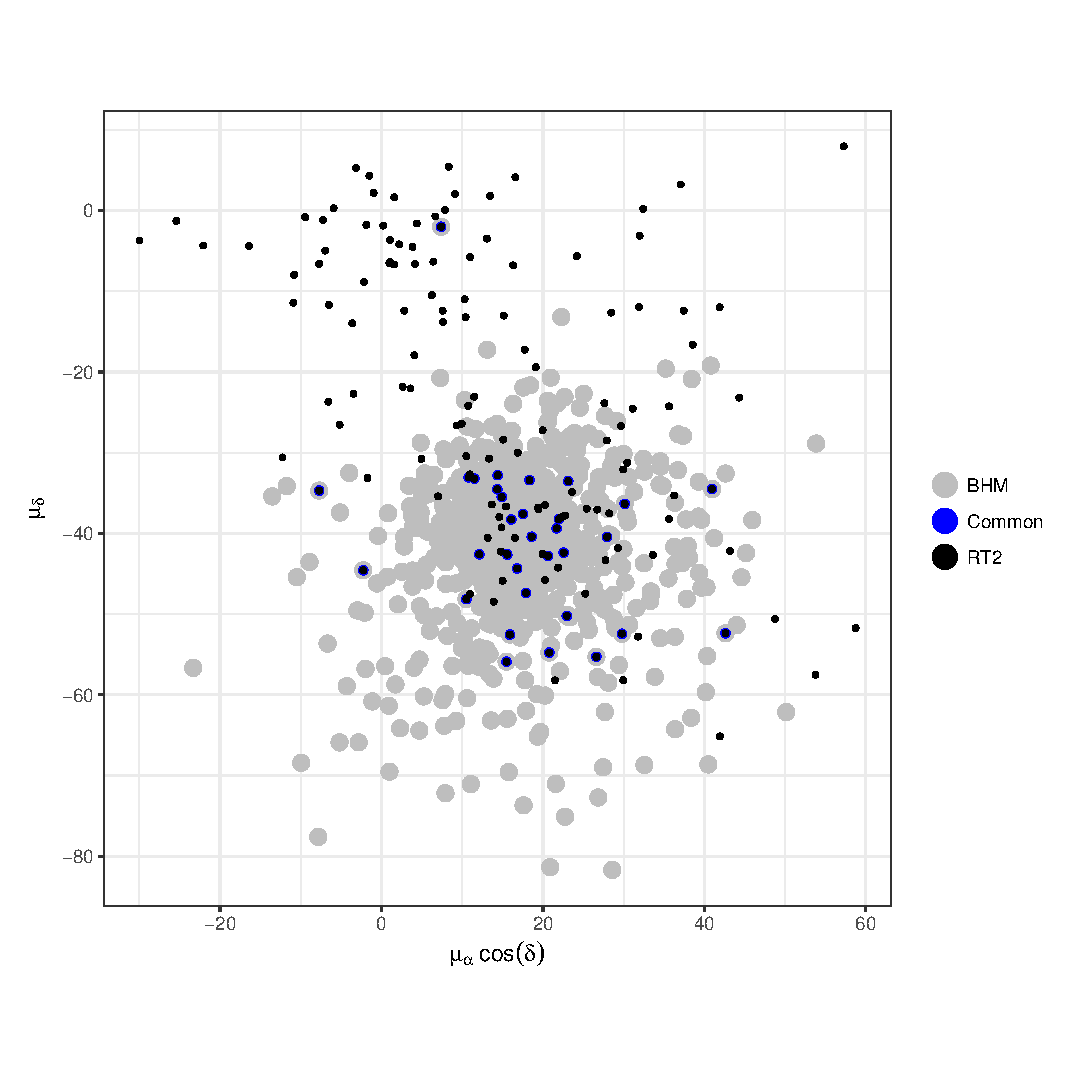
\includegraphics[width=\textwidth]{background/Figures/RT2_pm.eps}
        \caption{}
    \end{subfigure}
    \begin{subfigure}[t]{0.45\textwidth}
    \centering
     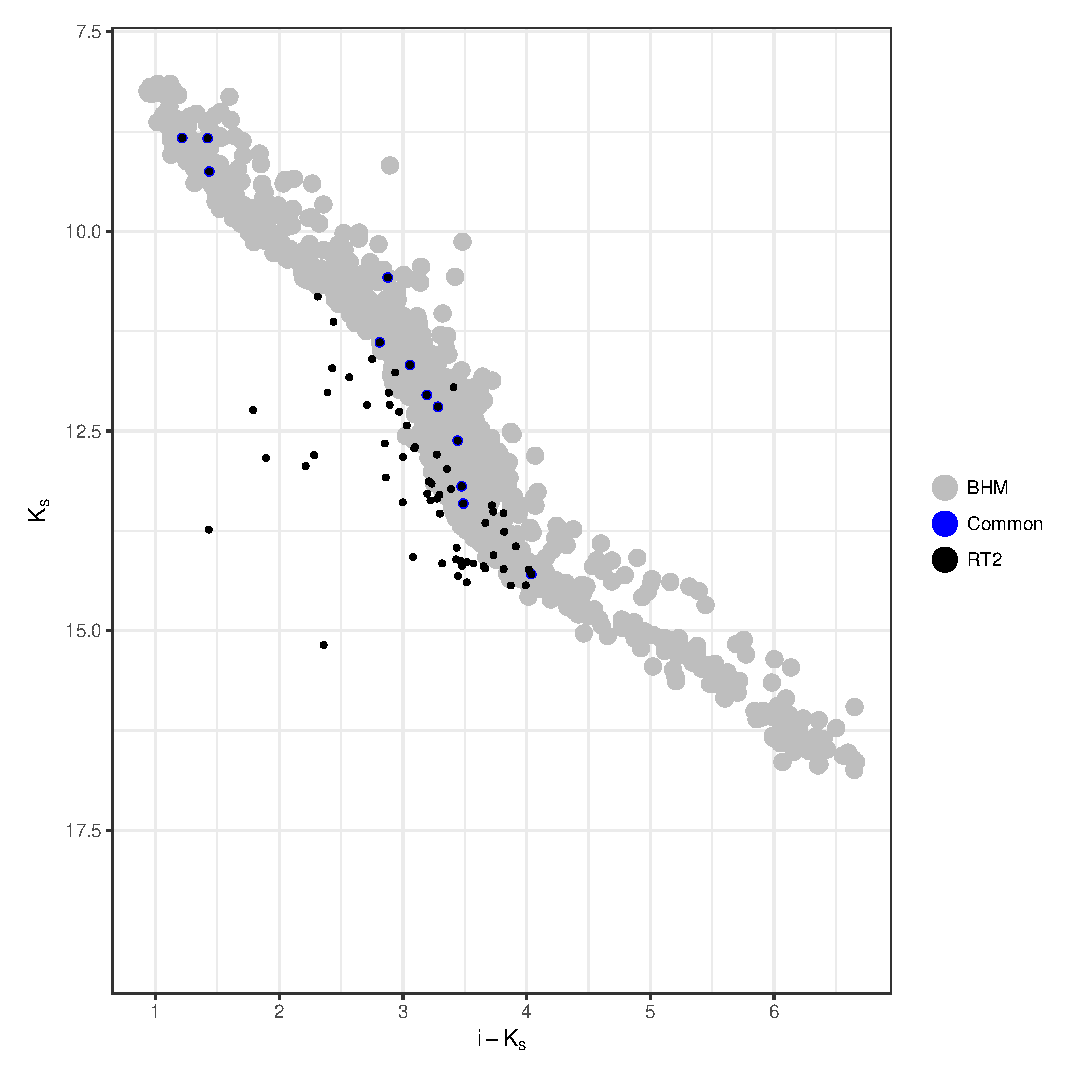
\includegraphics[width=\textwidth]{background/Figures/RT2_ph.eps}
        \caption{}
    \end{subfigure}
\caption{Proper motions (a) and $K$ vs $i-K$ \gls{cmd} (b) of the \gls{rt2} in the \gls{ddr2} catalogue (black). Also shown, the objects classified as candidate members in the \gls{bhm} (grey), and those classified as non-members in the \gls{rt2} and as candidate members in the \gls{bhm} (blue).}
\label{fig:RT2}
\end{figure}
 
\section{The statistical distributions of the Pleiades.}
Now, I present the results of the statistical distributions that describe the cluster population, which are the main objective of the present work. These distributions result directly or indirectly from the posterior distribution of the parameters in our model. Indirectly means that I use them as parameters of other function (e.g. the mass distribution). Since we have 85 parameters in the \gls{bhm}, I only discuss the posterior distributions of some of these parameters. In particular, those related with the velocity, luminosity and mass distributions. Nevertheless, in Table \ref{tab:parameters}, I summarise the posterior distribution of the parameters in our model using the mode, also I use the 16th and 84th percentiles as a proxy for the uncertainty. The parameter names in this Table correspond to those given in Section \ref{sect:priors} (at Table \ref{tab:priors_parameters}). 

\textbf{The posterior distributions of the parameters in the \glspl{bspline} and the \emph{true} \gls{ci} distribution are shown in Figs. \ref{fig:CMDs_results} and \ref{fig:CI_results}, respectively.  The posterior distributions of the parameters in the proper motion models are described in Section \ref{sect:PMresults}.}

\begin{figure}[ht!]
    \centering
    \begin{subfigure}[t]{0.48\textwidth}
        \includegraphics[page=7,height=8cm,width=\textwidth]{background/Figures/BHM/MembersModel.pdf}
        \caption{}
    \end{subfigure}
    \begin{subfigure}[t]{0.48\textwidth}
      \includegraphics[page=8,height=8cm,width=\textwidth]{background/Figures/BHM/MembersModel.pdf}
        \caption{}
    \end{subfigure}
     \begin{subfigure}[t]{0.48\textwidth}
      \includegraphics[page=9,height=8cm,width=\textwidth]{background/Figures/BHM/MembersModel.pdf}
        \caption{}   
    \end{subfigure}
     \begin{subfigure}[t]{0.48\textwidth}
      \includegraphics[page=10,height=8cm,width=\textwidth]{background/Figures/BHM/MembersModel.pdf}
        \caption{}
    \end{subfigure}
\caption{\glspl{cmd} showing the cluster (\gls{hmps}) and field members (blue triangles and grey dots, respectively resulting from classification using the $p_t = 0.84$ derived in Sect. \ref{sect:classifier}), together with 100 samples (orange spaghetti graphs) from the posterior distributions of the coefficients of the \glspl{bspline} resulting in the \emph{true} values of the cluster photometry. Also shown, the mode of these 100 samples (blue dashed line), the \gls{emb} sequence (magenta dot dashed line) and projections of the photometric field model (grey ellipses, see Fig. \ref{fig:fphGMM}).}
\label{fig:CMDs_results}
\end{figure}

\begin{figure}[ht!]
    \centering
      \includegraphics[page=1,width=\textwidth]{background/Figures/BHM/membersModel.pdf}
\caption{Posterior distribution of the \emph{true} \gls{ci} (orange lines, resulting from 100 samples of the posterior distributions of the parameters in the \gls{ci} \gls{gmm}). Also shown, the \gls{kde} (Gaussian kernel with bandwidth equal to observed uncertainty) for the observed \glspl{ci} of the candidate members in the \gls{hmps} (black line), and the prior distribution of the \emph{true} \gls{ci} \gls{gmm} (grey lines, resulting from 100 samples of the prior distributions of the parameters in the \gls{ci} \gls{gmm}).}
\label{fig:CI_results}
\end{figure}



Also, for the sake of completeness, in Fig. \ref{fig:correlations}, I depict the values the correlation coefficients among the 85 parameters in the \gls{bhm}. As can be seen from this Figure, the larger correlations appear among parameters describing the true $\gls{ci}$ distribution, and  among these and almost the rest of the parameters. This is expected since the true $\gls{ci}$ is key parameter in the \gls{bhm}. It is also interesting to notice that there is a strong correlation among the coefficients of the splines series modelling different magnitudes. For example, there is a strong correlation among the fourth coefficients of the splines. These correlations are expected since the shape of the cluster sequence is similar in the four \glspl{cmd}.  

\input{background/Tables/TableParameters.txt}

\begin{figure}[ht!]
\begin{center}
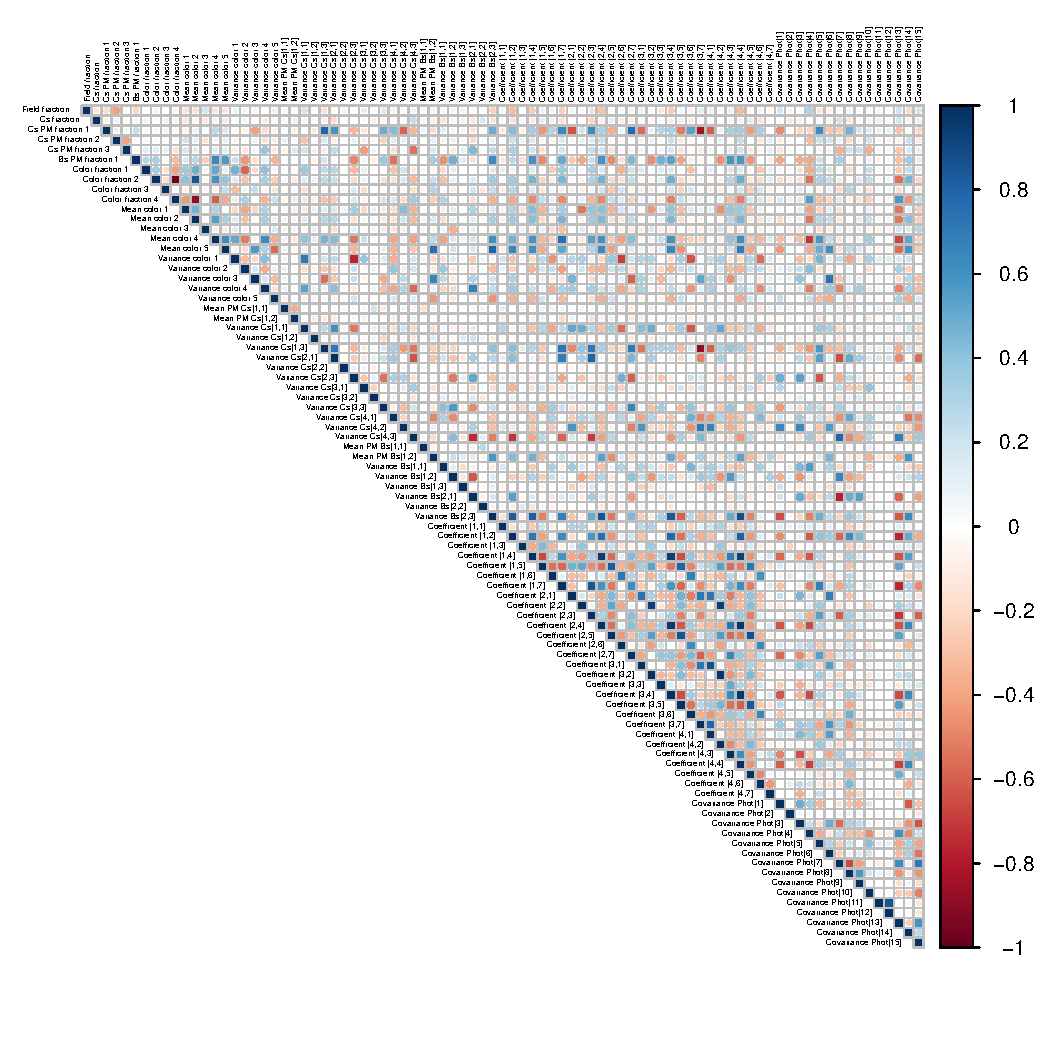
\includegraphics[page=1,width=1.1\textwidth]{background/Figures/BHM/Correlations.pdf}
\caption{Correlation matrix of the posterior distributions of the parameters in the \gls{bhm}. The colour code indicates the value of the correlation coefficient. Parameter names are the same as those in Table \ref{tab:parameters}.}
\label{fig:correlations}
\end{center}
\end{figure}

\section{Projected spatial distribution}
\label{sect:PSDresults}
In this Section, I present the results of the model selection analysis of the \glsfirst{psd} models of the Pleiades cluster. The Bayesian model selection approach and the \gls{psd} models are described in Sections \ref{sect:modelselection} and \ref{sect:PSDmethod}, respectively. The Bayesian \emph{evidence} is computed by means of the Python package \emph{PyMultiNest} \citep{Buchner2014}, which is a Python wrapper of the C++ package \emph{MultiNest} \citep{Feroz2009} that implements the Nested Sampling algorithm of \citet{Skilling2004,Skilling2006} (see Section \ref{sect:NestedSampling}).

Appendix \ref{app:posteriors} contains the details of the inference process 
of the posterior distributions, figures of the fitted densities and marginal distributions, 
together with the uncertainties of the parameters in each analysed model.
Table \ref{tab:BFAll}, given here, summarises the evidences and Bayes Factors
resulting for all our models and extensions. In the following we will use the figures in this Table to discuss the model comparison.


In the Bayesian model selection methodology, the boundaries for decision making from Bayes Factors should be set \emph{ab initio}. Thus, we discuss our results following the classical scale by \cite{Jeffreys61}, which I show in Table \ref{tab:JeffreysScale}.

\begin{table}[H]
\caption{\citet{Jeffreys61} scale for Bayes factors.}
\begin{center}
\begin{tabular}{cc}
Bayes factor & Strength of evidence\\
\hline
$\lesssim$ 3:1 & \emph{Inconclusive}\\
$\sim$ 3:1 & \emph{Weak}\\
$\sim$12:1 & \emph{Moderate}\\
$\gtrsim$ 150 :1 & \emph{Strong}\\
\hline
\end{tabular}
\end{center}
\label{tab:JeffreysScale}
\end{table}%
 

\begin{table*}
\tabcolsep=1pt
  \centering
  \caption[]{Natural logarithm of the evidence for each
        profile density (diagonal) and Bayes factors (off-diagonal
        elements, with the evidence for the model specified in the
        column header placed in the denominator). The evidence
        corresponds to data set truncated at 11.5pc.}  \label{tab:BFAll}
 \resizebox{\textwidth}{!}{
    \input{./Analysis/BayesFactors/BF_All_11_0.txt}
    }
  \end{table*}

\subsection{Selection of models with radial symmetry} 

The inferred posterior distributions of the parameters in our models with radial symmetry are shown in Fig. \ref{fig:PSDctr} by means of 100 samples randomly drawn, together with the \gls{map} value. For comparison, the data has been binned and is shown with poisson uncertainties.

\begin {figure}
\centering
\begin{subfigure}[t]{0.45\textwidth}
 \includegraphics[page=2,width=\textwidth]{Analysis/Centre/EFF_11/EFF_fit.pdf}
 \caption{EFF}  
    \end{subfigure}
    \begin{subfigure}[t]{0.45\textwidth}
 \includegraphics[page=2,width=\textwidth]{Analysis/Centre/GDP_11/GDP_fit.pdf}
 \caption{GDP}  
    \end{subfigure}
    \begin{subfigure}[t]{0.45\textwidth}
 \includegraphics[page=2,width=\textwidth]{Analysis/Centre/GKing_11/GKing_fit.pdf}
 \caption{GKing}  
    \end{subfigure}
    \begin{subfigure}[t]{0.45\textwidth}
 \includegraphics[page=2,width=\textwidth]{Analysis/Centre/King_11/King_fit.pdf}
 \caption{King}  
    \end{subfigure}
    \begin{subfigure}[t]{0.45\textwidth}
 \includegraphics[page=2,width=\textwidth]{Analysis/Centre/OGKing_11/OGKing_fit.pdf}
 \caption{OGKing}  
    \end{subfigure}
        \begin{subfigure}[t]{0.45\textwidth}
 \includegraphics[page=2,width=\textwidth]{Analysis/Centre/RGDP_11/RGDP_fit.pdf}
 \caption{RGDP}  
    \end{subfigure}
  \caption{Inferred density of the radially symmetric profiles shown by means of the \gls{map} value (red line) and samples from the posterior distribution (grey lines). 
  For comparison the data has been binned with poissonian uncertainties (black dots).}
\label{fig:PSDctr}
\end {figure}

The upper-left panel of Table \ref{tab:BFAll} summarises the evidences and Bayes
factors obtained from our radially symmetric models. In addition, Table \ref{tab:MAPCtr}, shows the \gls{map}
 estimate of each parameter in the radially symmetric models
(uncertainties are shown in the Appendix \ref{sect:app_radial} in the form of covariance matrices).
 
   
 \begin{table}[ht!]
  \centering
      \caption[]{Maximum-a-posteriori estimates of the inferred parameters in each radially symmetric model.}
         \label{tab:MAPCtr}
         \resizebox{\textwidth}{!}{
         \input{./Analysis/BayesFactors/MAPs_Centre_11.txt}
         }
   \end{table}
 
We observe that the evidences cluster in two groups. In one hand there is the family of King's
models, where the evidence to compare between them is inconclusive and moderate in favour of \gls{ogking} over \gls{gking}. 
On the other hand there are the \gls{eff}, \gls{gdp} and \gls{rgdp}, where there is moderate and weak evidence
supporting \gls{eff} over \gls{gdp} and \gls{rgdp}, respectively. \gls{rgdp} is moderately better than \gls{rgdp}.

Comparing the two groups shows that models in King's family have evidences that are: inconclusive and weak
over the \gls{eff}, weak and moderate over  \gls{rgdp}, and moderate over \gls{gdp}. Only from the evidences we can conclude that
the tidal radius is an important parameter.

In addition, we observe that in \gls{gdp} and \gls{rgdp}, the $r_c$ and $\beta$ parameters  show large correlations (0.85 and 0.92 for \gls{gdp} and \gls{rgdp}, respectively) and are relatively unconstrained with large uncertainties (see Appendix \ref{app:posteriors}).
Despite this fact, the models still have evidences comparable to those of the rest of the models. It suggests that these two parameters, although necessary for the model, are unconstrained by the data, and therefore not penalised by the evidence. Aiming at eliminating this source of degeneracy,
 we tested models in which one of these two parameters was removed. However, the fits and evidence resulting from
them were poorer than that of the \gls{rgdp}. Thus, we consider these parameters as necessary for this model.

We find that the introduction of more flexibility in the
analytical expressions of the classical radially symmetric profiles
does not produce larger evidences, and results in some cases in
unconstrained parameters and a loss of the interpretability associated
to the original formulations. Therefore, the best models are those pertaining to the King's family,
with not sufficient evidence to select which one of them is the best. Only
additional, perfectly acceptable prejudices like physical
interpretability or the ability to compare with previous results, can
be invoked to choose one (e.g. King's profile) over the rest.

The evidences seem 
to indicate that the best model is the \gls{ogking}.  
However, the fact that this profile has a larger evidence than any of the
remaining models should come as no surprise since it results from fixing
the values of $\alpha$ and $\beta$ of the \gls{gking} model to their MAP 
values. 

Comparing the rest of the models, we see that the poorest model is \gls{gdp} with moderate evidences against it. 
The best models are again in King's family followed by \gls{rgdp} and \gls{eff}.

The conclusion from the comparison of these radially symmetric
profiles is that i) there is no
compelling reason to abandon the widely used King profile in the
context of the complete and homogeneous data set,
and ii) there are slightly better models, but we lack evidence to prove if they truly 
represent a need to make the King's
profile more flexible to accommodate the data. 
In the following, we retain the models discussed above and
take the comparison one step further in order to include simple
deviations from radial symmetry in the form of elliptical density
contours.

\subsection{Selection of models with biaxial symmetry}

The inferred posterior distributions of the parameters in our models with biaxial symmetry are shown in Fig. \ref{fig:PSDEll} by means of 100 samples randomly drawn, together with the \gls{map} value. For comparison, the data has been binned and is shown with poisson uncertainties.

\begin {figure}
\centering
\begin{subfigure}[t]{0.45\textwidth}
 \includegraphics[page=2,width=\textwidth]{Analysis/Elliptic/EFF_11/EFF_fit.pdf}
 \caption{EFF}  
    \end{subfigure}
    \begin{subfigure}[t]{0.45\textwidth}
 \includegraphics[page=2,width=\textwidth]{Analysis/Elliptic/GDP_11/GDP_fit.pdf}
 \caption{GDP}  
    \end{subfigure}
    \begin{subfigure}[t]{0.45\textwidth}
 \includegraphics[page=2,width=\textwidth]{Analysis/Elliptic/GKing_11/GKing_fit.pdf}
 \caption{GKing}  
    \end{subfigure}
    \begin{subfigure}[t]{0.45\textwidth}
 \includegraphics[page=2,width=\textwidth]{Analysis/Elliptic/King_11/King_fit.pdf}
 \caption{King}  
    \end{subfigure}
    \begin{subfigure}[t]{0.45\textwidth}
 \includegraphics[page=2,width=\textwidth]{Analysis/Elliptic/OGKing_11/OGKing_fit.pdf}
 \caption{OGKing}  
    \end{subfigure}
        \begin{subfigure}[t]{0.45\textwidth}
 \includegraphics[page=2,width=\textwidth]{Analysis/Elliptic/RGDP_11/RGDP_fit.pdf}
 \caption{RGDP}  
    \end{subfigure}
  \caption{Inferred density of the biaxially symmetric profiles shown by means of the \gls{map} value (red line) and samples from the posterior distribution (grey lines). 
  For comparison the data has been binned with poissonian uncertainties (black dots).}
\label{fig:PSDEll}
\end {figure}

The central panel of  Table \ref{tab:BFAll} contains the
logarithm of the evidences and Bayes Factors of the biaxially symmetric models. The evidences follow a pattern similar to 
that observed for the radially symmetric models, with the exception of the evidences against the \gls{gdp} model. We can conclude that there is
strong evidence for the family of King's models agains the \gls{gdp} one.
The evidence is still moderate and weak to compare the rest of the models.

However, by comparing the evidences of the biaxially symmetric models to those of the radially symmetric ones (middle left panel of  Table \ref{tab:BFAll}), 
we can conclude that in all cases there is strong evidence in favour of the biaxial models.


Additionally, we compute a posteriori (from the \gls{mcmc} chains) the ellipticities\footnote{The ellipticity used here is also known as flattening.}  $\epsilon_{rc}$ and $\epsilon_{rt}$, which are defined as,

\begin{align}
\epsilon_{rc} = 1- \frac{r_{cb}}{r_{ca}}, \nonumber \\
\epsilon_{rt} = 1- \frac{r_{tb}}{r_{ta}}, \nonumber
\end{align}
with the latter available only for the King's family of models. 

 \begin{table*}[ht!]
  \centering
      \caption[]{Maximum-a-posteriori estimates of the inferred parameters in each biaxially symmetric model. Ellipticities are derived a posteriori using the inferred parameters.}
         \label{tab:MAPEll}
          \resizebox{\textwidth}{!}{
         \input{./Analysis/BayesFactors/MAPs_Elliptic_11.txt}
         }
   \end{table*}
   
Table \ref{tab:MAPEll} shows the MAP estimate of the parameters in the models of this section, together with the mode of the distributions of ellipticities. Uncertainties for the latter are given in Appendix \ref{sect:app_biaxial}.

We can observe that models that do not posses a tidal radius have similar $\epsilon_{rc}$ ellipticities with a mean value of $0.23\pm0.01$. This value is similar to the 0.17  found by \citep{Raboud1998}, who use a multicomponent analysis to derive the directions (although its value is not given) and the aspect ratio of the ellipse axes. However, it is very interesting to see that the models within King's family result in lower values of the ellipticity in the central region and larger values in the outer one. This result is expected from the interaction with the galactic potential and is predicted by the numerical simulations of open clusters \cite[see for example][]{1987MNRAS.224..193T}.

\subsection{Selection of models with luminosity segregation}
\label{sect:luminosity_segregation}
The inferred posterior distributions of the parameters in our models with biaxial symmetry and luminosity segregation are shown in Fig. \ref{fig:PSDSeg} by means of 100 samples randomly drawn, together with the \gls{map} value. For comparison, the data has been binned and is shown with poisson uncertainties. In addition, Fig. \ref{fig:Segregated} shows the density profiles of the luminosity segregated models, together with the J band data in three bins ($J < 12$, $12 \lesssim J \lesssim 15$, and $15 < J$). The three shown models have core radii as given by Eq. \ref{eq:rc_segregated}, in which the value of J band correspond to the mean of each bin.

\begin {figure}
\centering
\begin{subfigure}[t]{0.45\textwidth}
 \includegraphics[page=2,width=\textwidth]{Analysis/Segregated/EFF_11/EFF_fit.pdf}
 \caption{EFF}  
    \end{subfigure}
    \begin{subfigure}[t]{0.45\textwidth}
 \includegraphics[page=2,width=\textwidth]{Analysis/Segregated/GDP_11/GDP_fit.pdf}
 \caption{GDP}  
    \end{subfigure}
    \begin{subfigure}[t]{0.45\textwidth}
 \includegraphics[page=2,width=\textwidth]{Analysis/Segregated/GKing_11/GKing_fit.pdf}
 \caption{GKing}  
    \end{subfigure}
    \begin{subfigure}[t]{0.45\textwidth}
 \includegraphics[page=2,width=\textwidth]{Analysis/Segregated/King_11/King_fit.pdf}
 \caption{King}  
    \end{subfigure}
    \begin{subfigure}[t]{0.45\textwidth}
 \includegraphics[page=2,width=\textwidth]{Analysis/Segregated/OGKing_11/OGKing_fit.pdf}
 \caption{OGKing}  
    \end{subfigure}
        \begin{subfigure}[t]{0.45\textwidth}
 \includegraphics[page=2,width=\textwidth]{Analysis/Segregated/RGDP_11/RGDP_fit.pdf}
 \caption{RGDP}  
    \end{subfigure}
  \caption{Inferred density of the biaxially symmetric and luminosity segregated profiles shown by means of the \gls{map} value (red line) and samples from the posterior distribution (grey lines). 
  For comparison the data has been binned with poissonian uncertainties (black dots).}
\label{fig:PSDSeg}
\end {figure}

\begin {figure}
\centering
\begin{subfigure}[t]{0.45\textwidth}
 \includegraphics[page=5,width=\textwidth]{Analysis/Segregated/EFF_11/EFF_fit.pdf}
 \caption{EFF}  
    \end{subfigure}
    \begin{subfigure}[t]{0.45\textwidth}
 \includegraphics[page=5,width=\textwidth]{Analysis/Segregated/GDP_11/GDP_fit.pdf}
 \caption{GDP}  
    \end{subfigure}
    \begin{subfigure}[t]{0.45\textwidth}
 \includegraphics[page=5,width=\textwidth]{Analysis/Segregated/GKing_11/GKing_fit.pdf}
 \caption{GKing}  
    \end{subfigure}
    \begin{subfigure}[t]{0.45\textwidth}
 \includegraphics[page=5,width=\textwidth]{Analysis/Segregated/King_11/King_fit.pdf}
 \caption{King}  
    \end{subfigure}
    \begin{subfigure}[t]{0.45\textwidth}
 \includegraphics[page=5,width=\textwidth]{Analysis/Segregated/OGKing_11/OGKing_fit.pdf}
 \caption{OGKing}  
    \end{subfigure}
        \begin{subfigure}[t]{0.45\textwidth}
 \includegraphics[page=5,width=\textwidth]{Analysis/Segregated/RGDP_11/RGDP_fit.pdf}
 \caption{RGDP}  
    \end{subfigure}
  \caption{Density profiles of the data binned in J band ($J < 12$, green dots, $12 \lesssim J \lesssim 15$ cyan dots, and $15 < J$ magenta dots) together with the density models with parameters at the \gls{map} values. The core radii $r_c$ has been increased according to Eq. \ref{eq:rc_segregated}.}
\label{fig:Segregated}
\end {figure}

The lower-right panel of Table \ref{tab:BFAll} summarise the evidences and Bayes
Factors of models with luminosity segregation. Also, Table \ref{tab:MAPSg} shows the MAP of the inferred distributions for this set of models, together with the derived ellipticities.

\begin{table*}[ht!]
  \centering
      \caption[]{Maximum-a-posteriori estimates of the inferred parameters in each luminosity segregated model. Ellipticities are derived a posteriori using the inferred parameters.}
         \label{tab:MAPSg}
          \resizebox{\textwidth}{!}{
         \input{./Analysis/BayesFactors/MAPs_Segregated_11.txt}
         }
   \end{table*}
   
 We observe that the ellipticities follow the same pattern as those of the previous Section. This is expected because we explicitly model the luminosity segregation as independent of the position angle.
   
The luminosity segregation inferred here is non negligible with $\kappa$ in the range 0.1 to 0.25 $\rm{pc}\,\rm{mag}^{-1}$. Thus indicating that it is indeed an important parameter. However, in all the models, the marginal posterior distribution of $\kappa$ does not discard the zero value.

The evidences of the models with luminosity segregation follow a similar pattern as those from radial symmetry. However, in this case the best model is the classical King's, which shows only moderate evidences against the \gls{eff}, \gls{rgdp} and \gls{gdp} models. The evidence of King's model over \gls{gking} and O\gls{gking} is weak.

The evidences of the luminosity segregated models strongly favour them against the radially and biaxially symmetric ones in all cases. We can conclude that although with a small value of $\kappa$ the luminosity segregations is an important parameter regardless of the model used.




%%%%%%%%%%%%%%%%%%%%%%%%%%%%%%%%%%%%%%%%%%%%%%%%%%
\section{Proper motions distribution}
\label{sect:PMresults}
The bivariate proper motions distributions of both single and \gls{emb} is directly recovered by the \gls{bhm}. These bivariate distributions and their univariate projections, in the $\mu_{\alpha}\cdot cos(\delta)$ and $\mu_{\delta}$ components, are shown in Figs. \ref{fig:PM}, and,  \ref{fig:PMCs} and \ref{fig:PMBs}, respectively. These two latter figures also display the \gls{kde} of the proper motions of the candidate members in: i) \citet{Bouy2015}, and ii) the \gls{hmps}. Interestingly, the densities rendered by this two samples of candidate members are almost identical, except perhaps by the small excess of \citet{Bouy2015} in the region at  $\mu_{\delta}\sim -30$ mas yr$^{-1}$. 

Notice that, the density resulting from the \gls{bhm} differs from the \gls{kde} of the \gls{hmps}. I remember the reader that the \gls{bhm} recovers the posterior distribution of its parameters using the likelihood of all the objects in the data set (the $10^5$ in the \gls{rdr2}), with the contribution of individual objects proportional to their cluster membership probability. Therefore, the observed difference is the result of the two different samples of objects. The \gls{hmps} \gls{kde} uses only 1967 objects with cluster membership probability grater than 0.84, and not weighted by membership probability

\begin{figure}[ht!]
\begin{center}
\includegraphics[page=2,width=\textwidth]{background/Figures/BHM/MembersModel.pdf}
\caption{Proper motion distributions recovered by the \gls{bhm}. The dashed and dot-dashed ellipses represent the mode of 100 samples (orange lines) from the posterior covariance matrices in the cluster and \gls{emb} \glspl{gmm}, respectively. The grey ellipses depict the field model shown in panel (b) of Fig. \ref{fig:GMMvsMMM}. Reproduced from Figure 8 of \citet{Olivares2017},\textit{\usebibentry{Olivares2017}{Title}}, \usebibentry{Olivares2017}{Journal}, Vol. \usebibentry{Olivares2017}{Volume}.}
\label{fig:PM}
\end{center}
\end{figure}

\begin{figure}[ht!]
    \centering
    \begin{subfigure}[t]{0.45\textwidth}
    \centering
       \includegraphics[page=2,width=\textwidth]{background/Figures/BHM/Cs_members.pdf}
        \caption{}
    \end{subfigure}
    \begin{subfigure}[t]{0.45\textwidth}
    \centering
     \includegraphics[page=3,width=\textwidth]{background/Figures/BHM/Cs_members.pdf}
        \caption{}
    \end{subfigure}
\caption{Proper motions densities resulting from: a 100 element sample from the posterior distributions of parameters in the \gls{gmm} modelling the single stars (orange spaghetti lines), the kernel density estimation of the \gls{hmps} of candidate members classified as single stars (those whose cluster membership probability is higher than 0.84 and \gls{emb} membership probability is lower than 0.5), and, the kernel density estimation of the candidate members of \citet{Bouy2015} whose photometry lies below the \gls{emb} sequence (blue line).}
\label{fig:PMCs}
\end{figure}

\begin{figure}[ht!]
    \centering
    \begin{subfigure}[t]{0.45\textwidth}
    \centering
       \includegraphics[page=2,width=\textwidth]{background/Figures/BHM/Bs_members.pdf}
        \caption{}
    \end{subfigure}
    \begin{subfigure}[t]{0.45\textwidth}
    \centering
     \includegraphics[page=3,width=\textwidth]{background/Figures/BHM/Bs_members.pdf}
        \caption{}
    \end{subfigure}
\caption{Proper motions densities resulting from: a 100 element sample from the posterior distributions of parameters in the \gls{gmm} modelling the \gls{emb} stars (orange spaghetti lines), the kernel density estimation of the \gls{hmps} of candidate members classified as \gls{emb} stars (those whose cluster membership probability is higher than 0.84 and \gls{emb} membership probability is higher than 0.5), and, the kernel density estimation of the candidate members of \citet{Bouy2015} whose photometry lies near the \gls{emb} sequence (blue line).}
\label{fig:PMBs}
\end{figure}

Nevertheless, it is important to notice that, as the analysis of Section \ref{sect:classifier} indicates, objects with a missing \gls{ci} may have a biased membership probability, preferably towards higher values (see Fig. \ref{figure:IncVsCom}), and with a bias rms of 0.14. Thus, if I were to use a probability classification threshold of 0.5 instead of the 0.84 determined in Section \ref{sect:classifier}, the result will be a sample of  2907 candidate members whose \gls{kde} proper motion probability distribution would match that of the \gls{bhm} (see Fig. \ref{fig:PMCs>0.5}). From these 2907 hypothetical candidates, 50\% (1453) have a missing \gls{ci}. In contrast, using the correct probability threshold of 0.84 produces only 32\% (629) of candidates members with missing \gls{ci}. It is important to remark that not all objects with a missing \gls{ci} are biased. As estimated in Section \ref{sect:classifier} based on the synthetic data, the expected value of these contaminants all along the entire range of probability threshold is $5.8\pm 0.2$\%. Furthermore, the simulations with synthetic data, show no appreciable difference in the recovered proper motions distributions of objects with missing values when compared to those without them.

\begin{figure}[ht!]
    \centering
    \begin{subfigure}[t]{0.45\textwidth}
    \centering
       \includegraphics[page=3,width=\textwidth]{background/Figures/BHM/MembersModel_p>05.pdf}
        \caption{}
    \end{subfigure}
    \begin{subfigure}[t]{0.45\textwidth}
    \centering
     \includegraphics[page=4,width=\textwidth]{background/Figures/BHM/MembersModel_p>05.pdf}
        \caption{}
    \end{subfigure}
\caption{Proper motions densities resulting from: a 100 element sample from the posterior distributions of parameters in the \gls{gmm} modelling the single stars (orange spaghetti lines), the kernel density estimation of the hypothetical \gls{hmps} of objects with cluster membership probability grater than 0.5 and classified as single stars (red line).}
\label{fig:PMCs>0.5}
\end{figure}

The large wings in the proper motions distribution of the \gls{bhm} could be an effect of contamination, particularly because they are far from the cluster centre. However, proper motions and photometry have been independently modelled. Therefore, we have no reasons to believe that missing values affect predominately field objects with proper motions lying in this particular halo around the cluster centre. 

In contrast, due to mass segregation, the cluster members could be predominantly affected by missing values. If mass segregation were indeed present, as shown in Section \ref{sect:luminosity_segregation} with a luminosity proxy, then the fainter cluster members would be located in a halo around the cluster centre both in position and proper motions. This hypothesis is also supported by the lack of this effect in the proper motions distribution of \gls{emb} (see Fig. \ref{fig:PMBs}), this objects are massive than the average star, and therefore are brighter, less affected by missing values (at least in \gls{ci}), and due to the gravitational potential are located in the inner cluster region with lower proper motions. In any case, to taste the validity of this assumption we will have to wait the arrival of better data, with less missing values particularly.


\section{Luminosity distribution}
\label{sect:luminosity}
This Section describes the process to obtain the $J,H$, and $K_s$ absolute magnitude distributions from the posterior distributions of the parameters in the \gls{bhm}. Later, I compare them to those found by \citet{Bouy2015}, in the $K_s$ band specifically. As in the previous section, I also compare these distributions with those resulting from the kernel density estimates of the \gls{hmps} of candidate members resulting from the \gls{bhm}.

\subsection{Derivation of the magnitude distributions}
\label{subsect:deriveluminosity}

In the \gls{bhm} the photometric magnitudes are expressed as functions of the true $\gls{ci}$ (see Section \ref{subsect:cluster})
The $J,H,K_s$ magnitude distributions are derived by transforming the true $\gls{ci}$ distribution into the $J,H,K_s$ apparent magnitude distributions by means of the posterior distributions of the cluster photometric parameters. In particular, I use the \glspl{bspline} and the intrinsic dispersion of the cluster photometric sequence. In this transformations, the fractions of \gls{emb} are taken into account by mixing the single and \gls{emb} populations according to their fractions. In the following paragraphs, I describe the process to obtain the $K_s$ apparent magnitude. This process is similar for the rest of the bands. 

Since we aim at the probability distribution of $K_s$, and it depends on the true $\gls{ci}$, I use this as a nuisance parameter that I later marginalise. Thus, 

\begin{align}
p(K_s | \boldsymbol{\theta}_c) & = \int p(K_s,CI | \boldsymbol{\theta}_c) \cdot dCI =  \int p(K_s | CI ,\boldsymbol{\theta}_c) \cdot p(CI|\boldsymbol{\theta}_c)\cdot \mathrm{d}CI. \nonumber
\end{align}

The term $p(K_s | CI ,\boldsymbol{\theta}_c)$ represents the probability of $K_s$ given the true $\gls{ci}$ and the cluster parameters $\boldsymbol{\theta}_c$. It is given by Eq. \ref{eq:lik-seq}. The second term, $p(CI|\boldsymbol{\theta}_c)$ corresponds to the \gls{gmm} modelling the distribution of the true $\gls{ci}$, it is given by Eq. \ref{eq:colordist}. 

We include the \gls{emb}  distribution with an amplitude equal to their fraction, $1-\pi_{CB}$. Thus,

\begin{align}
p(K_s | \boldsymbol{\theta}_c) & =  \int \left[\pi_{CB}\cdot p_{Cs}(K_s| CI, \boldsymbol{\theta}_c) + (1-\pi_{CB})\cdot p_{Bs}(K_s| CI, \boldsymbol{\theta}_c)\right]\nonumber \\& \cdot p(CI|\boldsymbol{\theta}_c)\cdot \mathrm{d}CI. \nonumber \\
& =   \pi_{CB} \int p_{Cs}(K_s| CI, \boldsymbol{\theta}_c) \cdot p(CI|\boldsymbol{\theta}_c) \mathrm{d}CI \nonumber \\
&+ (1-\pi_{CB})\int p_{Bs}(K_s| CI, \boldsymbol{\theta}_c) \cdot p(CI|\boldsymbol{\theta}_c)\cdot  \mathrm{d}CI. \nonumber \\
\end{align}

In this equation, $Cs$ and $Bs$ are the subindices used to distinguish the probability of $K_s$ under the cluster and \gls{emb} photometric models, respectively. These probabilities are defined for the vector of photometric measurements, $\boldsymbol{d}_{ph}$ (see Eq. \ref{eq:lik-seq}). Since we are interested only in the distribution of $K_s$ (by now), we marginalise the rest of the photometric entries,including the observed $\gls{ci}$ (I use a tilde over the observed quantities). Also, the integration limits must change to those of the truncated true colour distribution ($\gls{ci}_{min}=0.8, \gls{ci}_{max}=8$). Hence,

\begin{align}
&p(K_s | \boldsymbol{\theta}_c)  =   \pi_{CB} \int_{CI_{min}}^{CI_{max}}\left[ \left[\sum_{i=1}^5 \pi_{CI,i} \cdot \mathcal{N}_t(CI| \mu_{CI,i},\sigma_{CI,i})\right]\right. \nonumber \\
&\cdot  \left.\int_{\tilde{CI},\tilde{Y},\tilde{J},\tilde{H}}\mathcal{N}(\{\tilde{CI},\tilde{Y},\tilde{J},\tilde{H},K_s\}|\boldsymbol{\mathcal{S}}(CI, \boldsymbol{\beta}),\Sigma_{clus})~\mathrm{d}\tilde{CI}~\mathrm{d}\tilde{Y}~\mathrm{d}\tilde{J}~\mathrm{d}\tilde{H}\right] \cdot \mathrm{d}CI \nonumber \\
& + (1-\pi_{CB}) \int_{CI_{min}}^{CI_{max}}\left[\left[\sum_{i=1}^5 \pi_{CI,i} \cdot \mathcal{N}_t(CI| \mu_{CI,i},\sigma_{CI,i})\right]\right.\nonumber\\
&\cdot \left. \int_{\tilde{CI},\tilde{Y},\tilde{J},\tilde{H}}\mathcal{N}(\{\tilde{CI},\tilde{Y},\tilde{J},\tilde{H},K_s\}|T_{Bs}(\boldsymbol{\mathcal{S}}(CI, \boldsymbol{\beta})),\Sigma_{clus})~\mathrm{d}\tilde{CI}~\mathrm{d}\tilde{Y}~\mathrm{d}\tilde{J}~\mathrm{d}\tilde{H}\right]\cdot \mathrm{d}CI. \nonumber 
\end{align}

The derivations of the $J$ and $H$ magnitude distributions are similar. Since this process takes into account the unresolved \gls{emb} and the so called single stars, which in fact could be binaries with low mass ratios, then I call these distributions the apparent system magnitude distributions. 

The previous distributions, together with the parallax and extinction of the cluster, are used to obtain the luminosity distributions, more properly the absolute system magnitude distributions. I assume that the distribution of parallaxes of the Pleiades members is normally distributed with mean, $7.44$ mas, and standard deviation $0.42$ mas \citep{Galli2017}. Then, to obtain the absolute magnitude distributions, I use the standard formulation
\begin{equation}
M = m - 5(\log_{10}{d} +1) = m + 5(\log_{10}\pi +1),\nonumber
\end{equation}

where $M$ and $m$ are the absolute and apparent magnitudes, and $d$ and $\pi$ the distance and parallax, respectively. Thus, I convolve the the distribution of the log parallax with the apparent $J,H,K_s$ magnitude distributions. Notice that here, for simplicity, I assume that the distribution of the parallax leads to the distribution of distances. Formally, the individual distances to the Pleiades must be inferred from the individual parallaxes  \cite[see for example][]{2016ApJ...833..119A}. Then the absolute magnitude distributions can be obtained by convolving this distance distribution with the apparent magnitude ones. Since the objective here is to compare the mass distribution with those in the literature, I proceed as in previous works and leave the formal treatment of distance inference to future works.

Finally, I deredden the previous distributions employing the canonical value of extinction for the Pleiades: $A_v=0.12$ mag \citep{Guthrie1987}. This last values were transformed into the $J,H,K_s$ extinctions using the extinction law of \citet{Cardelli1989}.

Since the \gls{bhm} describe the magnitudes as functions of the \gls{ci}, the completeness limits of the latter dictate those of the former, except for those of the $i$ and $K_s$ magnitude. The latter prescribe the completeness interval of the \gls{ci}, which is defined as that of all the points, along the cluster sequence in the $K_s$ vs. $i-K_s$ \gls{cmd}, for which $i$ and $K_s$ are bounded by their upper and lower completeness limits, respectively. Using the completeness limits found in Section \ref{sect:ddr2_completeness} results in a completeness interval of  $2.7<\gls{ci}<5.6$ mag. With it, and the cluster sequence (the splines and their parameters), I derive the completeness intervals for the $J,H,K_s$ bands. Finally, I transform these intervals to absolute magnitudes and deredden them. 

The luminosity distributions in the $J,H,K_s$ bands derived from the \gls{bhm}, together with their completeness limits are shown in Fig. \ref{fig:Luminosities}. For the sake of comparison, I also show the luminosity distributions resulting from the \gls{kde} in the magnitudes of the candidate members from: i) the \gls{hmps} derived in previous sections, and, ii)  \citet{Bouy2015}. Since the  luminosity distributions of Bouy and the \gls{hmps}, depend on the magnitudes of the individual candidate members, and many of them have missing entries, then I impute their missing values using those of the nearest euclidean neighbour. 

The difference between the luminosity distributions derived using the posterior distribution of the cluster photometric parameters (i.e. the \gls{bhm}) and that obtained from the \gls{hmps} of candidate members, comes as well from the fact that the \gls{hmps} is not a random sample of the cluster population, but it is selected based on the membership probability. Thus the latter is biased towards objects with high membership probability. Since the luminosity distributions derived from the cluster parameters takes into account all objects proportionally to their cluster membership probability, the it is free from this kind of bias. Another source of discrepancy comes from objects with missing entries. While in the luminosity resulting from the \gls{bhm} the missing values are marginalised, in that of the \gls{hmps} they are imputed.
 
On the other hand, the differences between the discrete distributions, the \gls{bhm} and that of \citet{Bouy2015}, arise mainly at the bright and faint ends ($K_s\sim 4$ mag and $K_s\sim11$ mag). I hypothesise that the origin of these differences lie in the different list of candidate members. To quantify the discrepancies between these two distributions, I performed the Anderson-Darling similarity test. In the comparison between the each of the 100 samples from the luminosity distribution from the \gls{bhm} and that of \citet{Bouy2015}, all the probabilities that the two distributions come from the same parent distributions are below $p< 0.04$ (the statistics from this test are in all cases larger than 10).

As it has been discussed, the model of \citet{Bouy2015} is constructed only based in fully observed objects. The regions where the objects with missing entries happen more frequently is in the bright and faint regions. Therefore, the observed differences in the luminosity distributions may arise from the simplistic treatment that those authors made of objects with missing entries (see Section \ref{sect:ignorability}).

\begin{figure}[htbp]
\begin{center}
\resizebox{\hsize}{!}{\includegraphics[width=0.8\textwidth]{background/Figures/BHM/absolute_JHK-log.pdf}}
\caption{Luminosity distribution of $J,H,K_s$ bands derived from the \gls{bhm} (orange spaghetti lines). Also shown: the regions of incompleteness, the luminosity distributions computed from: the candidate members of \citet{Bouy2015} (dot-dashed blue line), and our \gls{hmps} of candidate members, ($p_{84\%}>p_t$, dashed black line), and the prior for the true \gls{ci}, which was transformed in the same way as the posterior \gls{ci} distribution.}
\label{fig:Luminosities}.
\end{center}
\end{figure}

\section{Mass distribution}
\label{sect:massdistributionresults}

In this Section I describe the procedure to transform the luminosities distributions into mass distributions. Transforming a  probability distributions requires the transformation \emph{per se} and its derivative (see Section \ref{sect:introprobability}). Once the mass distributions is obtained,  then, I compare it to the \glspl{imf} of \citet{Chabrier2005} and \citet{Thies2007}. Finally, I conclude this section with the analysis of some simple toy models that can be fitted to the derived mass distribution.

\subsection{The mass-luminosity relation}
\label{sect:mass-luminosity}
The mass-luminosity relation is the non linear transformation that enables us to obtain the mass distribution from the luminosity distributions. Given the values of the upper limits of the luminosity distributions (the faint ends), the mass-luminosity relation relies entirely on the current models of stellar structure, where the atmospheres also play an important role. Among the different flavours of theoretical stellar evolution models in the literature (those from the Pisa, Padova, Trieste, Geneva, and Lyon research groups) we choose the BT-Settl models of \citet{Allard2012}. These models go deeper into the lower masses reaching the planetary mass range thus allowing a complete coverage of our luminosity distributions. The rest of the models stay in the $0.1-10\,\mathrm{M_{\odot}}$ range, with the \emph{PARSEC} models being the ones reaching the $0.1\,\mathrm{M_{\odot}}$ limit \citep{Bressan2012}.  Figure \ref{fig:BHM_vs_BT-Settl} compares the BT-Settl models of \citet{Allard2012} to the \gls{rdr2} data set (top panels), and to the cluster sequence obtained by the \gls{bhm} and the \gls{hmps} of cluster candidate members (bottom panels). The BT-Settl model corresponds to the Pleiades isochrone (at a distance of 134 pc, with 120 \gls{myr} and solar metallicity, which are the canonical ones, see Section \ref{sect:generalities}) given by the CIFIST2011bc grid, with $J$ and $K_s$ bands in the \gls{2mass} Vega photometric system and the $i$ band in the Sloan AB system, which correspond to the ones used in the \gls{ddr2} data set (H. Bouy, private communication).

Notice that the $i$ band photometry yielded by the BT-Settl model, contrary to the $J$ and $K_s$ ones, does not fit the observed data (solid lines in Fig. \ref{fig:BHM_vs_BT-Settl}). It must be shifted by 0.7 mag in order to be in accordance with the observed values (dashed lines in Fig. \ref{fig:BHM_vs_BT-Settl}). In a private communication with France Allard, she explained me that there was problem in the computation of some of the latest versions: a value from the earlier versions of \citet{1998A&A...337..403B} remained unaltered in the new versions. She assured me that they were working to solve that problem. This is probably the reason for the discrepant values returned by the Sloan AB system. However, since the the $J,H$ and $K_s$ bands are unaffected, this issue pose no problem for the further results of the present work. 

\begin{figure}[ht!]
    \centering
    \begin{subfigure}[t]{0.45\textwidth}
       \includegraphics[page=1,width=\textwidth]{background/Figures/BHM/BHM_vs_BT-Settl.pdf}
        \caption{}
    \end{subfigure}
    \begin{subfigure}[t]{0.45\textwidth}
     \includegraphics[page=2,width=\textwidth]{background/Figures/BHM/BHM_vs_BT-Settl.pdf}
        \caption{}
        \end{subfigure}
        \begin{subfigure}[t]{0.45\textwidth}
       \includegraphics[page=4,width=\textwidth]{background/Figures/BHM/BHM_vs_BT-Settl.pdf}
        \caption{}
    \end{subfigure}
    \begin{subfigure}[t]{0.45\textwidth}
     \includegraphics[page=6,width=\textwidth]{background/Figures/BHM/BHM_vs_BT-Settl.pdf}
        \caption{}
    \end{subfigure}
\caption{Comparison between observations and models. Top panels: $J$ vs. $K_s$ and $i$ vs $K_s$ magnitude-magnitude diagrams showing the \gls{rdr2} objects (black dots), and the original (green solid lines) and shifted (green dashed lines) BT-Settl models. Bottom panels: $J$ vs $i-K_s$ and $K_s$ vs $i-K_s$ \glspl{cmd} showing the \gls{hmps} of candidate members and the original (green solid lines) and shifted (green dashed lines) BT-Settl models. See text for details.}
\label{fig:BHM_vs_BT-Settl}
\end{figure}

The CIFIST2011bc grid returns values of the luminosity for certain non uniformly distributed values of the mass. As shown in Eq. \ref{eq:transformdistribution}, the transformation of a probability distribution, in this case the luminosities probability distributions, into the mass distribution is proportional to the derivative of the transformation, which must be continuous. To avoid the discontinuities in the derivatives produced by the grid, we fit the grid values by spline series (see Fig. \ref{fig:splineML}). Then, derivative is obtained from these continuous series (see Fig. \ref{fig:der_splineML}). It is important to notice the following two assumptions. First, I assume that the luminosity distributions in $J,H$ and $K_s$ bands are independent between them, and then I obtain a mass distribution for each one of them. Second, I assume that the transformation from luminosities to masses does not have any associated uncertainty. I must assume that because the isochrone models do not provide neither uncertainties nor a way to incorporate correlations between the mass distributions of distinct photometric bands. 

Figure \ref{fig:splineML} shows the spline fit to the mass-luminosity relations of the BT-Settl absolute $J,H$ and $K_s$ magnitudes (black points) as a function of the mass. Figure \ref{fig:der_splineML} shows the derivative of mass-luminosity relation. The grey shaded areas represent the incompleteness regions of the \gls{dance} survey (see previous section).

\begin{figure}[ht!]
    \centering
    \begin{subfigure}[t]{0.7\textwidth}
    \centering
       \includegraphics[page=1,width=\textwidth]{background/Figures/FitSpline_AllardModels.pdf}
        \caption{}
        \label{fig:splineML}
    \end{subfigure}
    \begin{subfigure}[t]{0.7\textwidth}
    \centering
     \includegraphics[page=2,width=\textwidth]{background/Figures/FitSpline_AllardModels.pdf}
        \caption{}
        \label{fig:der_splineML}
    \end{subfigure}
\caption{Upper panel: Mass-luminosity relations from the BT-Settl models \citep{Allard2012} for the $J, H$ and $K_s$ bands of the \emph{2MASS} photometric system (black dots). Also shown, the splines fitted to the previous relations. Bottom panel: The derivative of the mass-luminosity relations in the upper panel. The incompleteness regions of the \gls{dance} survey (grey areas) are shown in both panels.}
\label{fig:ML}
\end{figure}

\subsection{Present day system mass distribution}

The mass distribution is independently obtained for the $J,H,K_s$ luminosity distributions by means of the mass-luminosity relations described in the previous section. Since the luminosity functions of Sect. \ref{sect:luminosity} correspond to the luminosity of systems (single stars unresolved binaries and multiple systems), then, the derived mass function corresponds to the \glsfirst{pdsmd}.  Figure \ref{fig:MassDistribution} shows the logarithmic \gls{pdsmd} ($\xi_L$) for the $J,H,K_s$ bands normalised on the completeness limits of the \gls{ddr2}. The logarithmic representation of the mass distribution is a transformation from the natural variable of mass into the logarithm of 10 scale. It is customary to represent the mass distribution in this scale.

\begin{figure}[htbp]
\begin{center}
\resizebox{\hsize}{!}{\includegraphics[width=\textwidth]{background/Figures/BHM/MassDistribution.pdf}}
\caption{Normalised logarithmic \gls{pdsmd} in $J,H,K_s$ band. Also shown the completeness limits computed in previous section and transformed with the mass-luminosity relation, and the prior distribution, which was transformed in the same way as the posterior distribution.}
\label{fig:MassDistribution}
\end{center}
\end{figure}

The derived \gls{pdsmd} in $J,H,$ and $K_s$ bands are consistent with themselves for masses above 0.06 $M_{\odot}$ ($-1.2 < \log \mathrm{M/M_{\odot}}$). However, the $J$ band \gls{pdsmd} shows discrepancies with the $H$ and $K_s$ ones in the mass interval  $0.025 - 0.06 M_{\odot}$ ($-1.6 < \log \mathrm{M/M_{\odot}} < -1.2$), with a peak in discrepancy at 0.04$M_{\odot}$ ($-1.4 = \log \mathrm{M/M_{\odot}}$), see Fig. \ref{fig:MassDistribution}. The latter correspond to an effective temperature of $\sim$2200 K, which is at the middle of the transition between L and M dwarfs. This transition is not perfectly reproduced by any stellar structure and atmosphere model \citep{Allard2012}, and the BT-Settl one shows an excess in the flux of the $J$ band \citep{2013MmSAI..84.1053A}.

Due to the mentioned issue with the $J$ band, and the fact that the $K_s$ band is less affected by the interstellar extinction, in the following I will continue the discussion based only on the \gls{pdsmd} of this latter band.

For the sake of comparison, Figure \ref{fig:ModelMassFunction} shows the \gls{pdsmd} ($\xi_L$) for the $K_s$ band of the previous Figure, together with the three-slope power-law function of \citet{Bouy2015}, and the \gls{imf} of \citet{Thies2007} and \citet{Chabrier2005}. The standard uncertainties in \citet{Chabrier2005} \gls{imf} are those reported in \citet{Chabrier2003b}. 

This Figure shows that the \glspl{pdsmd} derived from the \gls{bhm} compare well, at least in the completeness interval, with the one proposed by \citet{Bouy2015}. The discrepancies between these two, above $0.3 \mathrm{M_{\odot}} (-0.5 < \log \mathrm{M/M_{\odot}})$ particularly, may have its origin on the following aspects.

The \gls{pdsmd} of \citet{Bouy2015} is computed using only their candidate members within the central three degree region of the \gls{ddr2}. First, their list of candidate members is not the same as those found by the \gls{bhm}. Second, the \gls{pdsmd} derived from the \gls{bhm} uses all objects in the data set, not just the high membership probability candidates. Third, as mentioned in Section \ref{sect:luminosity}, the cut to the central three degree region may have biased the derived \gls{pdsmd} of \citet{Bouy2015}. Therefore, the lack of objects that it shows,  in the mass range $0.3 - 0.7 \mathrm{M_{\odot}}$ ($-0.5 < \log \mathrm{M/M_{\odot}} < -0.2$) particularly, may has it origin in the objects that \citet{Bouy2015} did not included in his analysis: those lying outside the inner three degree region. 

For the sake of completeness, I fit a simple model to the \gls{pdsmd} obtained by the \gls{bhm}. To do it, I proceed as follows. First, I select three competing models: a log-normal function (like that of \citet{Chabrier2003b,Chabrier2005}), and two power-law functions of the form $m^{-\alpha}$ with two and three segments. Second, from the derived \gls{pdsmd} in the $K_s$ band, I took a sample of 100 distributions ( the ones shown as spaghetti lines in Fig. \ref{fig:ModelMassFunction}). Then, I divide  the completeness interval into a grid with 200 steps, and at each step I compute the mean of the values given by the 100 distributions. After normalisation this function can be thought as a mean distribution of the mass. Third, from the latter, I draw a sample of $10^4$ synthetic masses. Fourth, using \emph{PyMultiNest} \citep{Buchner2014} and the sample of synthetic masses, I obtain: i) the posterior distributions of the parameters in each of the three competing models, and ii) Bayesian evidences (Eq. \ref{eq:evidence}) for each of these models. In Table \ref{tab:fitPDSMD} I report the \gls{map} of the parameters in each model, together with the natural logarithm of the computed evidences. Judging by \citet{Jeffreys61} scale of evidence (see Table \ref{tab:JeffreysScale}), there is decisive evidence in favour of the two and three segment power-law models and against the log-normal function. However, the Bayes factor of the former indicates an evidence which barely worth mentioning. Under inconclusive evidence, I am allowed to use a simplicity prior (prejudice for simpler models) for the two competing power-law models (see Eq. \ref{eq:modelselection}). Thus, I chose the two-segment power-law model, which I show in Fig. \ref{fig:ModelMassFunction} by means of the black solid line.

The two segment power-law model agrees with the three segment model of \citet{Bouy2015}. However, there are still differences, which are clear at the low and high mass ends particularly. Nevertheless, it is in clear discrepancy with the \glspl{imf} of \citet{Chabrier2005},  \cite[$m_c=0.25_{-0.016}^{+0.021}$ and $\sigma=0.55_{-0.01}^{+0.05}$, the uncertainties are those reported by][for single objects]{Chabrier2003b} and of \citet{Thies2007}. 

The discrepancy between the \glspl{imf} and the \gls{pdsmd} derived from the \gls{bhm} and the \gls{pdsmd} of \citet{Bouy2015} may have its origin on the not yet established uncertainties in the mass-luminosity relation, on dynamical effects associated with age, or in a combination of the previous. In the next section I compare the \gls{pdsmd} of the Pleiades with that of other younger and older clusters in order to analyse if there is evidence of dynamical effects associated with age.

\begin{table*}[ht!]
\caption{Parameters and evidence of models fitted to the \gls{pdsmd}}
\begin{center}
\begin{tabular}{lll}
Model&Parameters& Log Evidence\\
\hline
LogNormal&$m_c=0.36\pm0.03$&\\
                 &$\sigma=0.46\pm0.02$ & $18.1 \pm 0.1$\\
\hline
Two Segments &$\alpha_0=-0.11\pm0.06$ \ \ $m \in [0.04,0.22\pm0.01]$ & \\ 
&  $\alpha_1=1.13\pm0.1$ \ \ $m \in [0.22\pm0.01,0.56]$&$2222.7\pm0.4$\\
\hline
Three Segments &$\alpha_0=-0.05\pm0.6$ \ \ $m \in [0.04,0.08\pm0.03]$ & \\
                          &$\alpha_1=-0.1\pm0.1$ \ \ $m \in [0.08\pm0.03,0.22\pm0.01]$ & \\ 
                          &$\alpha_2=1.13\pm0.1$ \ \ $m \in [0.22\pm0.01,0.56]$&$2221.2\pm 0.3$\\
\hline
\end{tabular}
\end{center}
\label{tab:fitPDSMD}
\end{table*}%

However, ending this section, I use the \gls{pdsmd} to give a lower limit to the mass of the cluster. Since the \gls{rdr2} data set  still lacks the very low mass range and most of the high mass range, the mass derived from this \gls{pdsmd} is only a lower limit to the mass of the cluster. From the \gls{pdsmd}, the cluster mean mass in the entire mass range is $0.257 \pm 0.006 \mathrm{M_{\odot}}$. Thus, the product of this mean mass with the expected number \footnote{As explained before, the expected number of cluster members is the integral, over the whole range of membership probabilities, of number of objects at each membership probability value.} of cluster members ($3301 \pm 140$), gives the expected mass of the cluster in this mass range. This  value is $845^{+38}_{-33} \mathrm{M_{\odot}}$. 

Finally, I notice that, as mentioned in Sect. \ref{sect:mass-luminosity}, the uncertainties in the mass-luminosity relations are yet to be established. Thus the quoted uncertainties of our mass results are underestimated.

\begin{figure}[htbp]
\begin{center}
\resizebox{\hsize}{!}{\includegraphics[page=1]{background/Figures/BHM/ModelsMassDistribution.pdf}}
\caption{Normalised logarithmic \gls{pdsmd} in $K_s$ band. Also shown the \glspl{imf} of \citet{Chabrier2005} \cite[blue dotted line with uncertainties from][]{Chabrier2003b} and  \citet{Thies2007} (turquoise long-dashed line), and power-law models found here (black solid line, see text) and by \citet{Bouy2015} (blue dashed line).}
\label{fig:ModelMassFunction}.
\end{center}
\end{figure}

\section{The mass distribution on time}
\label{sect:massontime}
Assuming the universality of the \gls{imf}, the observed differences between the present day mass distribution and the initial mass functions may have their origin on the temporal evolution of the cluster population. To test this hypothesis, I compare the Pleiades \gls{pdsmd} ($\sim125$ \gls{myr}) with those of the younger Trapezium \cite[0.2 to 1.4 \gls{myr}][]{Muench2002} and older Hyades \cite[$648 \pm 45$ \gls{myr}][]{DeGennaro2009} clusters. Under the assumption of a universal \gls{imf}, the \glspl{pdsmd} of these two cluster can be thought as snapshots of the Pleiades past and future mass distributions.

Although this comparison formally lies beyond the objectives of the present work, nevertheless, it gives an idea of the importance that the \gls{pdsmd} of other \gls{nyc} have in the understanding of the formation and evolution of the mass distribution.

Figure \ref{fig:PDSMDcomparison} shows the \gls{pdsmd} from the Pleiades, together with those of the Trapezium and Hyades\footnote{Kindly provided by Herv\'e Bouy in a private communication.}. These \glspl{pdsmd} correspond to those of  Fig. 11 of \citet{Bouy2015}. As mentioned by \citet{Bouy2015}, the abundance of low-mass stars and brown dwarfs in the range $0.03 - 0.1\,\mathrm{M_{\odot}}(-1.4 < \log \mathrm{M/M_{\odot}} <-1$) seems to diminish with time. The relative increase of objects in the range $-0.4 < \mathrm{\log M/M_{\odot}} < -0.2$ is an effect of the normalisation\footnote{The interesting alternative of open clusters gaining intermediate mass stars across their orbit is yet to be explored.}. This effect is consistent with the classical scenario in which low-mass stars and brown dwarfs are ejected as the cluster relaxes.

Since I lack the learned \gls{bhm} for these two open clusters, the following comparison is made on a frequentist hypothesis testing approach, rather than on the proper Bayesian model selection scheme.

In this hypothesis test, the null hypothesis is that the Hyades and Trapezium \glspl{pdsmd} came, each of them, from the same distribution than the Pleiades. 

If we want to test the null hypothesis that two distributions come from the same parent distribution, \gls{ks} and the \gls{ad} tests are classical options, with the \gls{ad} the most robust one. To perform these tests, we must compute certain measures from the two distributions. Then, given the measure, the test distribution returns the probability that the two distributions came from the same parent distribution. Finally, we reject the null hypothesis only if the previous probability is lower than certain probability threshold ($\alpha$), which is usually 0.1, 0.05, or 0.01. 

To perform the \gls{ks} tests we must obtain the maximum distance between the \glspl{cdf} of the two distributions. Then, using this distance and the \gls{ks} distribution, we obtain the probability that the two distributions came from the same parent distribution. %If this probability is higher than certain probability threshold ($\alpha$) then the null hypothesis can not be rejected. 

However, the \gls{ks} test can also be applied in a graphical way. Given the $\alpha$ probability threshold, there is a $d_{\alpha}$ distance for which the \gls{ks} distribution returns a probability $\alpha$. For $d < d_{\alpha}$ $p_{KS}(d) > \alpha$ and for $d > d_{\alpha}$ $p_{KS}(d) < \alpha$. Therefore, given the \gls{cdf} of one of the distributions that we want to compare and a probability threshold $\alpha$, the region of distance $d_{\alpha}$ around the \gls{cdf} depicts the hypothesis test. If the \gls{cdf} of the other distribution lies entirely within this region, then its maximum distance from the first \gls{cdf} is less than $d_{\alpha}$. Therefore, its probability is greater than $\alpha$ and the null hypothesis can not be rejected.

\begin{figure}[htp]
\begin{center}
\resizebox{\hsize}{!}{\includegraphics[width=\textwidth]{background/Figures/BHM/M45vsM42vsM44.pdf}}
\caption{The \glspl{pdsmd} of the Pleiades (derived here for $J,H,K_s$ bands), Trapezium, and Hyades (both from \citet{Bouy2015}) clusters. They are normalised in the interval of completeness.}
\label{fig:PDSMDcomparison}.
\end{center}
\end{figure}

\begin{figure}[htp]
\begin{center}
\resizebox{\hsize}{!}{\includegraphics[width=\textwidth]{background/Figures/BHM/CDF_comparison.pdf}}
\caption{\glspl{cdf} of the \glspl{pdsmd} from left panel and that of \citet{Chabrier2005} and \citet{Thies2007} system initial mass function (normalised also in the interval of completeness). The shown Pleiades \gls{cdf} correspond to the $K_s$ band. The grey area depicts the area in which the \glspl{cdf} (both Trapezium and Hyades) should lie for the null hypothesis not to be rejected (at $\alpha=0.01$).}
\label{fig:PDSMDtest}
\end{center}
\end{figure}


Figure \ref{fig:PDSMDtest} shows the cumulative distribution functions (\glspl{cdf}) of the Trapezium, Pleiades (in $K_s$ band) and Hyades \glspl{pdsmd}. Also and for comparison, I show the \glspl{cdf} resulting of \citet{Chabrier2005} and \citet{Thies2007} \glspl{imf}. The grey area around the Pleiades \gls{cdf} depicts the graphical \gls{ks} hypothesis test in which I choose $\alpha = 0.01$.

Furthermore, since the \gls{ks} test uses only the maximum distance between \glspl{cdf}, I also applied the more robust \gls{ad} test. It also rejects the null hypotheses (at $p < 0.004$) that the Trapezium and Hyades \glspl{pdsmd} and the \citet{Chabrier2005} and \citet{Thies2007} \glspl{imf} came from the same parent distribution as the Pleiades \gls{pdsmd}. 

The previous tests suggest that there is enough statistical evidence  to support the diverse origins in the \glspl{pdsmd} of these three clusters. Also, these evidences suggest that \glspl{imf} of \citet{Chabrier2005} and \citet{Thies2007} are statistically different from the  Pleiades \gls{pdsmd}.  These observed differences, as mentioned in the previous Section, may have its origin on dynamical effects associated with age and relaxation. However, they can also arise due to the simpler assumption that no two clusters are born alike.

Whatever the answer to this question is, to obtain it, at least two issues must be solved. 
First, the uncertainties in the \gls{pdsmd} must be properly established, particularly those of the mass-luminosity relation, distance, and extinction. Here, I have assumed that i) extinction is a single value instead of a distribution of values, ii) distance is the inverse of the parallax, which underestimates the uncertainties, and, iii) the mass-luminosity is a unique transformation, which in fact must be a set of transformations that must take into account the age spread and metallicities of clusters, and possible discrepancies amongst stellar structure models.

Second, the luminosity distributions of all compared clusters must include the properly propagated uncertainties from the data, as in the \gls{bhm}, and not just from the poissonian counts as in those of the Trapezium and Hyades. Thus, in the future, the \gls{bhm} of the remaining clusters must be computed. 

Once this issues are solved, the \glspl{bhm} of different clusters will allow us to gauge how similar these clusters are. Indeed, by comparing the posterior \glspl{pdf} of the model parameters returned by the data sets of different clusters, given the same model and set of assumptions, we would be able to properly measure, by means of hypothesis tests \cite[see for example][]{Rueda1992}, the probability that these models were drawn from the same parent \gls{pdf}. 

\section{Updating priors and assumptions}
\label{sect:updating_priors}
As mentioned by \citet{Gelman2006}, the posterior distribution must be inspected to update our previous knowledge. To inspect these posterior distribution, I use the statistics reported in Table \ref{tab:parameters}. These values indicate, for example, that the number of  \gls{gmm} modelling the proper motions of the single stars is overestimated. The fraction and variance of the last gaussian are both to near zero values. Probably, a better model would be that in which the parameters of these extra gaussian will not be part of the model. Ideally, I should select one of these two models based on their evidence (see Section \ref{sect:modelselection}). To my knowledge, the only reliable approach to compute the evidence of a model inferred using \gls{mcmc}, is by means of the Nested Sampling algorithm (see Section \ref{sect:NestedSampling}). However, running the \gls{bhm} in the \emph{MultiNest} package lies far beyond our current computational resources.

The following are two examples of posterior checking that were performed in the iterative cycle of model and inference. 

In a past run of the \gls{bhm} on the \gls{rdr2}, I realised that the prior distribution for the parameter modelling field fraction was too narrow. Although the maximum of the posterior distribution was allowed by this prior (by definition), the prior density at this \gls{map} was negligible. Therefore, I updated the prior to a distribution with a larger variance, thus weakening the prior information. As can be seen from Fig. \ref{fig:fractions}, the posterior distribution of the $\pi$ and $\pi_{CB}$ fraction parameters in the \gls{bhm} are now allowed by the prior distributions. It is important to notice that, given the large information provided by the data, the prior distributions play a small roll in the estimation of the posterior (i.e. the likelihood is highly informative). 

\begin{figure}[ht!]
\begin{center}
\includegraphics[page=1,width=0.45\textwidth]{background/Figures/BHM/Fractions.pdf}
\includegraphics[page=2,width=0.45\textwidth]{background/Figures/BHM/Fractions.pdf}
\caption{Posterior distributions of the $\pi$ and $\pi_{CB}$ parameters (orange lines) together with their corresponding priors. Notice that due to the large data set, the posterior distributions are highly concentrated.}
\label{fig:fractions}
\end{center}
\end{figure}

In the first version of this manuscript, the evidences for the \gls{psd} models presented in Section \ref{sect:PSDresults} were computed using uniform priors for all parameters. As kindly pointed out by Coryn Bailer-Jones, one of the referees of this work, the truncation limits of those priors have an influence on the estimated evidences. By modifying those priors and allowing them to \textit{reflect the available parameter space under the model $\mathcal{M}$, independently of experimental constraints we might already be aware of} \cite[taken from][]{Trotta2008}, we were able to measure the simplicity (evidence) of the model itself. 

\subsection{Assumptions}
The posterior checking not only must be performed on the inferred parameters but also in the model itself. In such spirit, this section describes how two key assumptions in the field model have been modified by our posterior inference.



Finally, I hope that this last Section has transmitted the reader how dynamic, iterative and reflexive the creation of a model is. While the Bayesian formalism enable us to update our prior knowledge based on the data, transform it into posteriors, and select the best models based on evidence, the Bayesian Hierarchical approach allows us to directly update our prior beliefs within the inference process. In summary, the Bayesian formalism help us to update our knowledge based not just in the light of new data, but also in the light of new models.
 




